\chapter{Results} % Main chapter title

\label{Results}

%----------------------------------------------------------------------------------------
%	SECTION 1
%----------------------------------------------------------------------------------------
This chapter presents findings from the experiments on task-incremental instruction fine-tuning, addressing the research questions posed in Chapter \ref{Introduction}. Through these experiments, the effect of sequential LoRA-based parameter efficient fine-tuning was examined on both Code Generation and Natural Language Generation use cases. The results are organized into two separate sections. The first section presents the results from our experiments with Code Generation use case. The results from the different fine-tuning sequences listed in Table \ref{tab:CodeTaskOrder} are presented for both the baseline and mitigation settings. The second section presents the results from our experiments with Natural Language Generation use case. In this section, the results from the fine-tuning sequences listed in Table \ref{tab:GenTaskOrder} are presented for both the baseline and mitigation settings. This encompasses the experiments carried out to investigate the impact of task-incremental learning and task order on the retention of model's pre-trained and task-specific learned capabilities. 

Throughout this chapter, shorter representations for the task names and evaluations have been used to account for their frequent use.
\\

\begin{tabular}{ll}
\textbf{Full name} & \textbf{Representation used} \\
\hline
Evaluation & \\
\hspace{1em} Pre-evaluation stage & pre\_eval \\
\hspace{1em} Post evaluation after 1st model fine-tune & post\_eval1 \\
\hspace{1em} Post evaluation after 2nd model fine-tune & post\_eval2 \\
\hspace{1em} Post evaluation after 3rd model fine-tune & post\_eval3 \\
Code Generation tasks & \\
\hspace{1em} Code Generation in C++ & cg \\
\hspace{1em} Unit Test Generation & utg \\
\hspace{1em} Manifest Generation & mg \\
Natural Language Generation tasks & \\
\hspace{1em} Question Answering & qa \\
\hspace{1em} Summarization & summ \\
\hspace{1em} Mathematical Reasoning & math \\
\end{tabular}

\section{Code Generation use case}
This section presents the results from the experiments carried out with Code Generation use case tasks: cg, utg, and mg. Evaluation with different benchmarks and task-specific assessments have been conducted to measure and track the changes in the pre-trained capabilities of the instruct model across fine-tunes. 

\subsection{Evaluation of model's pre-trained capabilities}
The results from the pre-evaluation stage performance of the DeepSeek-Coder-6.7B-Instruct model on HumanEval (+ MultiPL-E) and CoNaLa benchmarks and task-specific evaluations are presented in Table \ref{tab:CodeBenchmarkPreEval} and Table \ref{tab:CodeTaskEvalPreEval} respectively. The results presented have been averaged across two runs.

%----Table 1
% \begin{table}[h!]
% \centering
% \caption{Performance of DeepSeek-Coder-6.7B-Instruct on different benchmarks}
% \begin{tabular}{|l|l|l|l|}
% \hline
% Evaluation Benchmark & Dataset & Score & Metric \\
% \hline
% \multirow{3}{*}{HumanEval (+ MultiPL-E)} & C++ & 0.6375 & \multirow{3}{*}{pass@1} \\
% & Java & 0.64375 & \\
% & Python & 0.76875 & \\
% \hline
% CoNaLa & CoNaLa & 0.216249 & CodeBLEU \\
% \hline
% \end{tabular}
% \label{tab:CodeBenchmarkPreEval}
% \end{table}

\begin{table}[H]
\centering
\caption{Performance of DeepSeek-Coder-6.7B-Instruct on different benchmarks}
\begin{tabular}{lllllll}
\hline
\multicolumn{1}{|l|}{Evaluation   Benchmark}                    & \multicolumn{1}{l|}{Metric}                                                & \multicolumn{1}{l|}{Dataset} & \multicolumn{1}{l|}{Total Size} & \multicolumn{1}{l|}{N} & \multicolumn{1}{l|}{Score}  & \multicolumn{1}{l|}{Reported Score} \\ \hline
\multicolumn{1}{|c|}{}                                          & \multicolumn{1}{l|}{{\color[HTML]{467886} }}                               & \multicolumn{1}{l|}{C++}     & \multicolumn{1}{l|}{161}        & \multicolumn{1}{l|}{80}              & \multicolumn{1}{l|}{0.6375} & \multicolumn{1}{l|}{0.634}          \\ \cline{3-7} 
\multicolumn{1}{|c|}{}                                          & \multicolumn{1}{l|}{{\color[HTML]{467886} }}                               & \multicolumn{1}{l|}{Java}    & \multicolumn{1}{l|}{158}        & \multicolumn{1}{l|}{80}              & \multicolumn{1}{l|}{0.6438} & \multicolumn{1}{l|}{0.684}          \\ \cline{3-7} 
\multicolumn{1}{|c|}{\multirow{-3}{*}{HumanEval (+ MultiPL-E)}} & \multicolumn{1}{l|}{\multirow{-3}{*}{{pass@1}}} & \multicolumn{1}{l|}{Python}  & \multicolumn{1}{l|}{164}        & \multicolumn{1}{l|}{80}              & \multicolumn{1}{l|}{0.7688} & \multicolumn{1}{l|}{0.786} \\ \hline
\multicolumn{1}{|c|}{CoNaLa   (CodeBLEU)}                       & \multicolumn{1}{l|}{CodeBLEU}                                              & \multicolumn{1}{l|}{CoNaLa}  & \multicolumn{1}{l|}{500}        & \multicolumn{1}{l|}{100}             & \multicolumn{1}{l|}{0.2162} & \multicolumn{1}{l|}{}               \\ \hline
\end{tabular}
\label{tab:CodeBenchmarkPreEval}
\end{table}


% %-----Table 2
% \begin{table}[h!]
% \centering
% \caption{Performance of DeepSeek-Coder-6.7B-Instruct on Test and Validation datasets for different tasks}
% \begin{tabular}{|l|l|r|}
% \hline
% Task & Dataset & Score (CodeBLEU) \\
% \hline
% \multirow{2}{*}{cg} & Test & 0.046312 \\
%  & Validation & 0.041909 \\
% \hline
% \multirow{2}{*}{utg} & Test & 0.114348 \\
%  & Validation & 0.152672 \\
% \hline
% \multirow{2}{*}{mg} & Test & 0.034924 \\
%  & Validation & 0.036390 \\
% \hline
% \end{tabular}
% \label{tab:CodeTaskEvalPreEval}
% \end{table}

\begin{table}[H]
\centering
\caption{Performance of DeepSeek-Coder-6.7B-Instruct on Test and Validation datasets for different tasks}
\begin{tabular}{clll}
\cline{1-4}
\multicolumn{1}{|l|}{Task}                 & \multicolumn{1}{l|}{Dataset}    & \multicolumn{1}{l|}{Sample size (N)} & \multicolumn{1}{l|}{Score (CodeBLEU)} \\ \cline{1-4}
\multicolumn{1}{|c|}{\multirow{2}{*}{cg}}  & \multicolumn{1}{l|}{Test}       & \multicolumn{1}{l|}{500}             & \multicolumn{1}{l|}{0.0463}          \\ \cline{2-4}
\multicolumn{1}{|c|}{}                     & \multicolumn{1}{l|}{Validation} & \multicolumn{1}{l|}{501}             & \multicolumn{1}{l|}{0.0419}           \\ \cline{1-4}
\multicolumn{1}{|c|}{\multirow{2}{*}{utg}} & \multicolumn{1}{l|}{Test}       & \multicolumn{1}{l|}{48}              & \multicolumn{1}{l|}{0.1143}           \\ \cline{2-4}
\multicolumn{1}{|c|}{}                     & \multicolumn{1}{l|}{Validation} & \multicolumn{1}{l|}{48}              & \multicolumn{1}{l|}{0.1527}           \\ \cline{1-4}
\multicolumn{1}{|c|}{\multirow{2}{*}{mg}}  & \multicolumn{1}{l|}{Test}       & \multicolumn{1}{l|}{145}             & \multicolumn{1}{l|}{0.0349}           \\ \cline{2-4}
\multicolumn{1}{|c|}{}                     & \multicolumn{1}{l|}{Validation} & \multicolumn{1}{l|}{146}             & \multicolumn{1}{l|}{0.0364}           \\ \cline{1-4}
\multicolumn{1}{l}{}                       &                                 &                                      &                                       \\
\multicolumn{1}{l}{}                       &                                 &                                      &                                       \\
\multicolumn{1}{l}{}                       &                                 &                                      &                                      
\end{tabular}
\label{tab:CodeTaskEvalPreEval}
\end{table}

The results on the benchmark datasets showed that our evaluation scores are relatively close scores to the reported scores for the HumanEval (+MultiPL-E) benchmark. The model was found to perform the best on the Python dataset, which could indicate the model has strong capabilities in Python.

\subsection{Baseline experiment results}
The baseline experiments were carried out by performing sequential task-incremental instruction fine-tuning without the use of replay. The results from the experiments on benchmark evaluations and task-specific performance evaluations are presented in Table \ref{tab:CodeBaselineCombined}. The presented results have been averaged across two seed values and the six different fine-tuning sequences for the task order.
\begin{table}[H]
\centering
\caption{Benchmarks and Task-specific evaluation results for Baseline runs of Code Generation use case}
\begin{tabular}{|c|l|l|l|l|l|l|}
\hline
\multicolumn{1}{|l|}{\textbf{Evaluation}}  & \textbf{Dataset} & \textbf{N} & \textbf{pre\_eval} & \textbf{post\_eval1} & \textbf{post\_eval2} & \textbf{post\_eval3} \\ \hline
\multirow{3}{*}{HumanEval   (+ MultiPL-E)} & C++              & 80         & 0.6375             & 0.4583               & 0.4854               & 0.4313               \\ \cline{2-7} 
                                           & Java             & 80         & 0.6438             & 0.5354               & 0.4427               & 0.3833               \\ \cline{2-7} 
                                           & Python           & 80         & 0.7688             & 0.6958               & 0.6094               & 0.6448               \\ \hline
CoNaLa                                     & CoNaLa           & 100        & 0.2162             & 0.2178               & 0.2101               & 0.2027               \\ \hline
\multirow{2}{*}{cg}                        & Test             & 500        & 0.0463             & 0.0754               & 0.1137               & 0.1392               \\ \cline{2-7} 
                                           & Validation       & 501        & 0.0419             & 0.0766               & 0.1146               & 0.1379               \\ \hline
\multirow{2}{*}{utg}                       & Test             & 48         & 0.1143             & 0.1073               & 0.1133               & 0.1145               \\ \cline{2-7} 
                                           & Validation       & 48         & 0.1527             & 0.1508               & 0.1583               & 0.1658               \\ \hline
\multirow{2}{*}{mg}                        & Test             & 145        & 0.0349             & 0.0335               & 0.0463               & 0.0541               \\ \cline{2-7} 
                                           & Validation       & 146        & 0.0364             & 0.0295               & 0.0390               & 0.0444               \\ \hline
\end{tabular}
\label{tab:CodeBaselineCombined}
\end{table}


% \begin{table}[h!]
% \centering
% \caption{Benchmarks and Task-specific evaluation results for Baseline runs of Code Generation use case}
% \begin{tabular}{|l|l|r|r|r|r|}
% \hline
% Evaluation & Dataset & pre\_eval & post\_eval1 & post\_eval2 & post\_eval3 \\
% \hline
% \multirow{3}{*}{HumanEval (+ MultiPL-E)} & C++ & 0.6375 & 0.458333 & 0.485417 & 0.43125 \\
% \cline{2-6}
% & Java & 0.64375 & 0.535417 & 0.442708 & 0.383333 \\
% \cline{2-6}
% & Python & 0.76875 & 0.695833 & 0.609375 & 0.644792 \\
% \hline
% CoNaLa & CoNaLa & 0.216249 & 0.217774 & 0.210067 & 0.202716 \\
% \hline
% \multirow{2}{*}{cg} & Test & 0.046312 & 0.075411 & 0.113695 & 0.139169 \\
% \cline{2-6}
% & Validation & 0.041909 & 0.076567 & 0.114612 & 0.13788 \\
% \hline
% \multirow{2}{*}{utg} & Test & 0.114348 & 0.107345 & 0.113327 & 0.114511 \\
% \cline{2-6}
% & Validation & 0.152672 & 0.150773 & 0.158349 & 0.165846 \\
% \hline
% \multirow{2}{*}{mg} & Test & 0.034924 & 0.033462 & 0.046339 & 0.054133 \\
% \cline{2-6}
% & Validation & 0.03639 & 0.029505 & 0.039047 & 0.044422 \\
% \hline
% \end{tabular}
% \label{tab:CodeBaselineCombined}
% \end{table}
% \begin{table}[!ht]
    \centering
    \caption{Performance on the C++ dataset of HumanEval (+ MultiPL-E) benchmark across ablations for Baseline runs}
    \begin{tabular}{|l|l|S[table-format=2.4]|S[table-format=2.4]|S[table-format=2.4]|S[table-format=2.4]|}
    \hline
        \textbf{Ablation} & \textbf{Task order} & \textbf{pre\_eval} & \textbf{post\_eval1} & \textbf{post\_eval2} & \textbf{post\_eval3 } \\ \hline
        Ablation 1 & cg-utg-mg & 0.6375 & 0.525 & 0.4625 & 0.45625  \\ 
        Ablation 2 & cg-mg-utg & 0.6375 & 0.525 & 0.50625 & 0.43125  \\ 
        Ablation 3 & utg-cg-mg & 0.6375 & 0.30625 & 0.55 & 0.48125  \\ 
        Ablation 4 & utg-mg-cg & 0.6375 & 0.30625 & 0.38125 & 0.38125  \\ 
        Ablation 5 & mg-cg-utg & 0.6375 & 0.54375 & 0.50625 & 0.45  \\ 
        Ablation 6 & mg-utg-cg & 0.6375 & 0.54375 & 0.50625 & 0.3875 \\ \hline
    \end{tabular}
    \label{tab:CppBaseline}
\end{table}

\begin{table}[!ht]
    \centering
    \caption{Performance on the Java dataset of HumanEval (+ MultiPL-E) benchmark across ablations for Baseline runs}
    \begin{tabular}{|l|l|S[table-format=2.4]|S[table-format=2.4]|S[table-format=2.4]|S[table-format=2.4]|}
    \hline
        \textbf{Ablation} & \textbf{Task order} & \textbf{pre\_eval} & \textbf{post\_eval1} & \textbf{post\_eval2} & \textbf{post\_eval3 } \\ \hline
        Ablation 1 & cg-utg-mg & 0.64375 & 0.5 & 0.475 & 0.2625  \\ 
        Ablation 2 & cg-mg-utg & 0.64375 & 0.5 & 0.325 & 0.3875  \\ 
        Ablation 3 & utg-cg-mg & 0.64375 & 0.54375 & 0.575 & 0.33125  \\ 
        Ablation 4 & utg-mg-cg & 0.64375 & 0.54375 & 0.4 & 0.475  \\ 
        Ablation 5 & mg-cg-utg & 0.64375 & 0.5625 & 0.40625 & 0.34375  \\ 
        Ablation 6 & mg-utg-cg & 0.64375 & 0.5625 & 0.475 & 0.5 \\ \hline
    \end{tabular}
    \label{tab:JavaBaseline}
\end{table}

\begin{table}[!ht]
    \centering
    \caption{Performance on the Python dataset of HumanEval (+ MultiPL-E) benchmark across ablations for Baseline runs}
    \begin{tabular}{|l|l|S[table-format=2.4]|S[table-format=2.4]|S[table-format=2.4]|S[table-format=2.4]|}
    \hline
        \textbf{Ablation} & \textbf{Task order} & \textbf{pre\_eval} & \textbf{post\_eval1} & \textbf{post\_eval2} & \textbf{post\_eval3 } \\ \hline
        Ablation 1 & cg-utg-mg & 0.76875 & 0.66875 & 0.6125 & 0.65  \\ 
        Ablation 2 & cg-mg-utg & 0.76875 & 0.66875 & 0.65625 & 0.6375  \\ 
        Ablation 3 & utg-cg-mg & 0.76875 & 0.7 & 0.64375 & 0.65625  \\ 
        Ablation 4 & utg-mg-cg & 0.76875 & 0.7 & 0.6875 & 0.675  \\ 
        Ablation 5 & mg-cg-utg & 0.76875 & 0.71875 & 0.41875 & 0.5875  \\ 
        Ablation 6 & mg-utg-cg & 0.76875 & 0.71875 & 0.6375 & 0.6625 \\ \hline
    \end{tabular}
    \label{tab:PythonBaseline}
\end{table}

\begin{table}[!ht]
    \centering
    \caption{Performance on the CoNaLa benchmark across ablations for Baseline runs}
    \begin{tabular}{|l|l|S[table-format=2.4]|S[table-format=2.4]|S[table-format=2.4]|S[table-format=2.4]|}
    \hline
        \textbf{Ablation} & \textbf{Task order} & \textbf{pre\_eval} & \textbf{post\_eval1} & \textbf{post\_eval2} & \textbf{post\_eval3 } \\ \hline
        Ablation 1 & cg-utg-mg & 0.216249 & 0.212248 & 0.21981 & 0.2039585  \\ 
        Ablation 2 & cg-mg-utg & 0.216249 & 0.212248 & 0.209731 & 0.198182  \\ 
        Ablation 3 & utg-cg-mg & 0.216249 & 0.220624 & 0.210697 & 0.2047265  \\ 
        Ablation 4 & utg-mg-cg & 0.216249 & 0.220624 & 0.213846 & 0.206291  \\ 
        Ablation 5 & mg-cg-utg & 0.216249 & 0.2204505 & 0.197515 & 0.2002515  \\ 
        Ablation 6 & mg-utg-cg & 0.216249 & 0.2204505 & 0.2088005 & 0.202889 \\ \hline
    \end{tabular}
    \label{tab:CoNaLaBaseline}
\end{table}

\begin{table}[!ht]
    \centering
    \caption{Performance on the Test set of Code Generation in C++ task across ablations for Baseline runs}
    \begin{tabular}{|l|l|S[table-format=2.4]|S[table-format=2.4]|S[table-format=2.4]|S[table-format=2.4]|}
    \hline
        \textbf{Ablation} & \textbf{Task order} & \textbf{pre\_eval} & \textbf{post\_eval1} & \textbf{post\_eval2} & \textbf{post\_eval3 } \\ \hline
        Ablation 1 & cg-utg-mg & 0.0463115 & 0.1349755 & 0.1361555 & 0.138237  \\ 
        Ablation 2 & cg-mg-utg & 0.0463115 & 0.1349755 & 0.1371045 & 0.1271735  \\ 
        Ablation 3 & utg-cg-mg & 0.0463115 & 0.0374325 & 0.152484 & 0.1472625  \\ 
        Ablation 4 & utg-mg-cg & 0.0463115 & 0.0374325 & 0.0601475 & 0.150081  \\ 
        Ablation 5 & mg-cg-utg & 0.0463115 & 0.0538245 & 0.1391325 & 0.133467  \\ 
        Ablation 6 & mg-utg-cg & 0.0463115 & 0.0538245 & 0.0571485 & 0.1387905 \\ \hline
    \end{tabular}
    \label{tab:CodeGenTestBaseline}
\end{table}

\begin{table}[!ht]
    \centering
    \caption{Performance on the Validation set of Code Generation in C++ task across ablations for Baseline runs}
    \begin{tabular}{|l|l|S[table-format=2.4]|S[table-format=2.4]|S[table-format=2.4]|S[table-format=2.4]|}
    \hline
        \textbf{Ablation} & \textbf{Task order} & \textbf{pre\_eval} & \textbf{post\_eval1} & \textbf{post\_eval2} & \textbf{post\_eval3 } \\ \hline
        Ablation 1 & cg-utg-mg & 0.0419085 & 0.142302 & 0.1274795 & 0.126582  \\ 
        Ablation 2 & cg-mg-utg & 0.0419085 & 0.142302 & 0.1423165 & 0.12579  \\ 
        Ablation 3 & utg-cg-mg & 0.0419085 & 0.037424 & 0.1552265 & 0.144193  \\ 
        Ablation 4 & utg-mg-cg & 0.0419085 & 0.037424 & 0.052555 & 0.1480245  \\ 
        Ablation 5 & mg-cg-utg & 0.0419085 & 0.049976 & 0.1527795 & 0.1394835  \\ 
        Ablation 6 & mg-utg-cg & 0.0419085 & 0.049976 & 0.057314 & 0.1432045 \\ \hline
    \end{tabular}
    \label{tab:CodeGenValBaseline}
\end{table}

\begin{table}[!ht]
    \centering
    \caption{Performance on the Test set of Unit Test Generation in task across ablations for Baseline runs}
    \begin{tabular}{|l|l|S[table-format=2.4]|S[table-format=2.4]|S[table-format=2.4]|S[table-format=2.4]|}
    \hline
        \textbf{Ablation} & \textbf{Task order} & \textbf{pre\_eval} & \textbf{post\_eval1} & \textbf{post\_eval2} & \textbf{post\_eval3 } \\ \hline
        Ablation 1 & cg-utg-mg & 0.1143475 & 0.100622 & 0.124755 & 0.1105215  \\ 
        Ablation 2 & cg-mg-utg & 0.1143475 & 0.100622 & 0.0982835 & 0.1211765  \\ 
        Ablation 3 & utg-cg-mg & 0.1143475 & 0.129741 & 0.114616 & 0.106551  \\ 
        Ablation 4 & utg-mg-cg & 0.1143475 & 0.129741 & 0.1133925 & 0.108431  \\ 
        Ablation 5 & mg-cg-utg & 0.1143475 & 0.091671 & 0.095757 & 0.1324305  \\ 
        Ablation 6 & mg-utg-cg & 0.1143475 & 0.091671 & 0.133159 & 0.107954 \\ \hline
    \end{tabular}
    \label{tab:UnitTestGenTestBaseline}
\end{table}

\begin{table}[!ht]
    \centering
    \caption{Performance on the Validation set of Unit Test Generation in task across ablations for Baseline runs}
    \begin{tabular}{|l|l|S[table-format=2.4]|S[table-format=2.4]|S[table-format=2.4]|S[table-format=2.4]|}
    \hline
        \textbf{Ablation} & \textbf{Task order} & \textbf{pre\_eval} & \textbf{post\_eval1} & \textbf{post\_eval2} & \textbf{post\_eval3 } \\ \hline
        Ablation 1 & cg-utg-mg & 0.1526715 & 0.1356135 & 0.17702 & 0.15221  \\ 
        Ablation 2 & cg-mg-utg & 0.1526715 & 0.1356135 & 0.129706 & 0.172063  \\ 
        Ablation 3 & utg-cg-mg & 0.1526715 & 0.192541 & 0.1709965 & 0.156134  \\ 
        Ablation 4 & utg-mg-cg & 0.1526715 & 0.192541 & 0.158679 & 0.163308  \\ 
        Ablation 5 & mg-cg-utg & 0.1526715 & 0.1241635 & 0.133897 & 0.180247  \\ 
        Ablation 6 & mg-utg-cg & 0.1526715 & 0.1241635 & 0.179795 & 0.1711145 \\ \hline
    \end{tabular}
    \label{tab:UnitTestGenValBaseline}
\end{table}

\begin{table}[!ht]
    \centering
    \caption{Performance on the Test set of Manifest Generation in task across ablations for Baseline runs}
    \begin{tabular}{|l|l|S[table-format=2.4]|S[table-format=2.4]|S[table-format=2.4]|S[table-format=2.4]|}
    \hline
        \textbf{Ablation} & \textbf{Task order} & \textbf{pre\_eval} & \textbf{post\_eval1} & \textbf{post\_eval2} & \textbf{post\_eval3 } \\ \hline
        Ablation 1 & cg-utg-mg & 0.034924 & 0.039671 & 0.0376915 & 0.051237  \\ 
        Ablation 2 & cg-mg-utg & 0.034924 & 0.039671 & 0.054898 & 0.0519355  \\ 
        Ablation 3 & utg-cg-mg & 0.034924 & 0.0070935 & 0.0238505 & 0.0548525  \\ 
        Ablation 4 & utg-mg-cg & 0.034924 & 0.0070935 & 0.0528435 & 0.0580775  \\ 
        Ablation 5 & mg-cg-utg & 0.034924 & 0.0536225 & 0.054903 & 0.057162  \\ 
        Ablation 6 & mg-utg-cg & 0.034924 & 0.0536225 & 0.053846 & 0.051532 \\ \hline
    \end{tabular}
    \label{tab:ManifestGenTestBaseline}
\end{table}

\begin{table}[!ht]
    \centering
    \caption{Performance on the Validation set of Manifest Generation in task across ablations for Baseline runs}
    \begin{tabular}{|l|l|S[table-format=2.4]|S[table-format=2.4]|S[table-format=2.4]|S[table-format=2.4]|}
    \hline
        \textbf{Ablation} & \textbf{Task order} & \textbf{pre\_eval} & \textbf{post\_eval1} & \textbf{post\_eval2} & \textbf{post\_eval3 } \\ \hline
        Ablation 1 & cg-utg-mg & 0.0363895 & 0.036197 & 0.035644 & 0.0447165  \\ 
        Ablation 2 & cg-mg-utg & 0.0363895 & 0.036197 & 0.043876 & 0.04471  \\ 
        Ablation 3 & utg-cg-mg & 0.0363895 & 0.0075775 & 0.022038 & 0.0437745  \\ 
        Ablation 4 & utg-mg-cg & 0.0363895 & 0.0075775 & 0.0437745 & 0.044901  \\ 
        Ablation 5 & mg-cg-utg & 0.0363895 & 0.0447415 & 0.043907 & 0.043902  \\ 
        Ablation 6 & mg-utg-cg & 0.0363895 & 0.0447415 & 0.0450425 & 0.0445295 \\ \hline
    \end{tabular}
    \label{tab:ManifestGenValBaseline}
\end{table}


From the results of the baseline experiments, it was observed that the performance scores of the model on the benchmark datasets declined over time. The performance on C++ and Java datasets of the HumanEval (+ MultiPL-E) benchmark suffered the most with a decline from 0.63 to 0.43 and from 0.64 to 0.38 respectively from the pre-evaluation stage to the final post-evaluation stage. This degradation of performance over time showed forgetting of the pre-trained capabilities of the model on these tasks. There was a decline in performance for the Python set of the HumanEval (+ MultiPL-E) benchmark. However, the performance on the CoNaLa benchmark remained relatively steady throughout the fine-tunes.

For the task-specific evaluations, there was a gradual improvement in the task performance for all tasks, with Code Generation in C++ task having the highest improvement from 0.04 to 0.13 in both the test and validation sets. 

The degradation of model performance on the benchmark datasets over time showed forgetting of the model’s pre-trained capabilities after task-specific fine-tuning and showed the need for mitigation methods to be put in place to prevent catastrophic forgetting. The improvement in task-specific performance for all the tasks demonstrated that the model was learning new task-specific capabilities across fine-tunes.


\subsubsection{Mitigation experiment results}
The mitigation experiments were carried out by performing sequential instruction fine-tuning with the use of replay as a mitigation step for catastrophic forgetting. The results from the mitigation experiments on benchmark evaluations and task-specific performance evaluations are presented in Table \ref{tab:TraceMitigationCombined}. The presented results have been averaged across two seed values and the six different fine-tuning sequences for different task orders.
\begin{table}[H]
\centering
\caption{Benchmarks and Task-specific evaluation results for Mitigation runs of Code Generation use case}
\begin{tabular}{|c|l|l|l|l|l|l|}
\hline
\multicolumn{1}{|l|}{\textbf{Evaluation}}  & \textbf{Dataset} & N   & \textbf{pre\_eval} & \textbf{post\_eval1} & \textbf{post\_eval2} & \textbf{post\_eval3} \\ \hline
\multirow{3}{*}{HumanEval   (+ MultiPL-E)} & C++              & 80  & 0.6375             & 0.5375               & 0.4927               & 0.4521               \\ \cline{2-7} 
                                           & Java             & 80  & 0.6438             & 0.5313               & 0.4740               & 0.4042               \\ \cline{2-7} 
                                           & Python           & 80  & 0.7688             & 0.6875               & 0.6167               & 0.6167               \\ \hline
CoNaLa                                     & CoNaLa           & 100 & 0.2162             & 0.2200               & 0.2165               & 0.2041               \\ \hline
\multirow{2}{*}{cg}                        & Test             & 500 & 0.0463             & 0.0847               & 0.1258               & 0.1558               \\ \cline{2-7} 
                                           & Validation       & 501 & 0.0419             & 0.0813               & 0.1198               & 0.1576               \\ \hline
\multirow{2}{*}{utg}                       & Test             & 48  & 0.1143             & 0.1108               & 0.1189               & 0.1272               \\ \cline{2-7} 
                                           & Validation       & 48  & 0.1527             & 0.1588               & 0.1685               & 0.1821               \\ \hline
\multirow{2}{*}{mg}                        & Test             & 145 & 0.0349             & 0.0475               & 0.0484               & 0.0539               \\ \cline{2-7} 
                                           & Validation       & 146 & 0.0364             & 0.0414               & 0.0415               & 0.0443               \\ \hline
\end{tabular}
\label{tab:CodeMitigationCombined}
\end{table}



% \begin{table}[htbp]
% \centering
% \caption{Benchmarks and Task-specific evaluation results for Mitigation runs of Code Generation use case}
% \begin{tabular}{|p{4.5cm}|l|r|r|r|r|}
% \hline
% Evaluation & Dataset & pre\_eval & post\_eval1 & post\_eval2 & post\_eval3 \\
% \hline
% \multirow{3}{*}{HumanEval (+ MultiPL-E)} & C++ & 0.6375 & 0.5375 & 0.492708 & 0.452083 \\
% \cline{2-6}
% & Java & 0.64375 & 0.53125 & 0.473958 & 0.404167 \\
% \cline{2-6}
% & Python & 0.76875 & 0.6875 & 0.616667 & 0.616667 \\
% \hline
% CoNaLa & CoNaLa & 0.216249 & 0.219995 & 0.216476 & 0.204121 \\
% \hline
% \multirow{2}{*}{cg} & Test & 0.046312 & 0.084672 & 0.125814 & 0.155808 \\
% \cline{2-6}
% & Validation & 0.041909 & 0.081297 & 0.119771 & 0.157552 \\
% \hline
% \multirow{2}{*}{utg} & Test & 0.114348 & 0.110808 & 0.118915 & 0.127154 \\
% \cline{2-6}
% & Validation & 0.152672 & 0.158781 & 0.168485 & 0.182078 \\
% \hline
% \multirow{2}{*}{mg} & Test & 0.034924 & 0.047484 & 0.048441 & 0.053857 \\
% \cline{2-6}
% & Validation & 0.03639 & 0.041367 & 0.041492 & 0.044294 \\
% \hline
% \end{tabular}
% \label{tab:CodeMitigationCombined}
% \end{table}
% \input{Chapters/ResultsSubpages/CodeMitigationResults}

The results from the mitigation runs showed that the performance scores on the benchmark datasets declined over the task-incremental fine-tunes. This indicated that there was still loss of the model's pre-trained capabilities even with the addition of the mitigation step.
For the task-specific evaluations, similar to baseline experiments, a gradual performance improvement was observed for all tasks. 

\subsection{Baseline vs Mitigation performance}
To understand the impact of replay on the retention of the model's pre-trained and task-specific capabilities, we compared the model's performance between the baseline and mitigation runs. 

\subsubsection{Impact on model's pre-trained capabilities}
In this section, we compare the performance of the model on the benchmark datasets between the baseline and mitigation runs.
\begin{figure}[H]
    \centering
    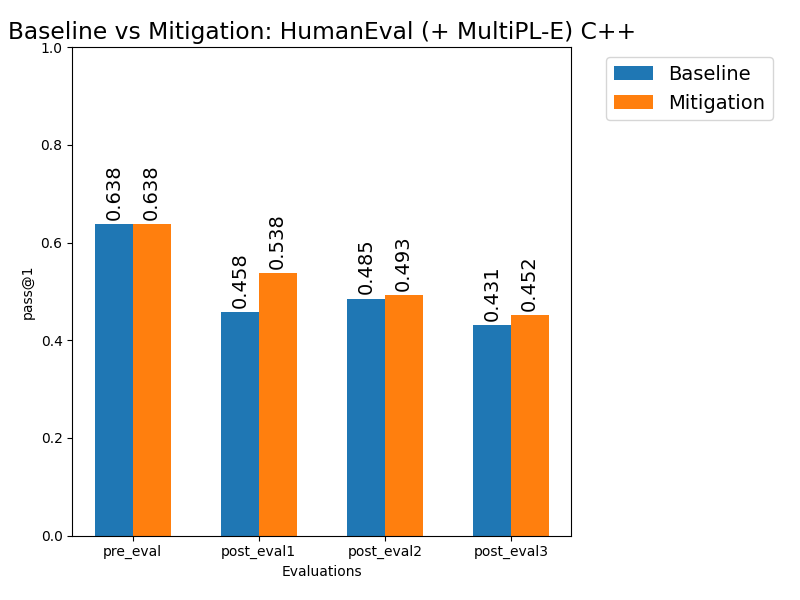
\includegraphics[width=0.8\textwidth]{Figures/results/code_comparisons/human_eval/comparison_humaneval_cpp.png} 
    \caption{Baseline vs. Mitigation for HumanEval (+ MultiPL-E) C++}
    \label{fig:CppComparison}
\end{figure}
The comparison of the performance on the HumanEval (+MultiPL-E) C++ benchmark showed that in both the baseline and mitigation runs, there was notable decline in model performance across the different post-evaluation stages. The addition of replay mitigation offered a slight improvement in the performance in post\_eval1. However, this improvement was not sustained in the subsequent fine-tunes.

\begin{figure}[H]
    \centering
    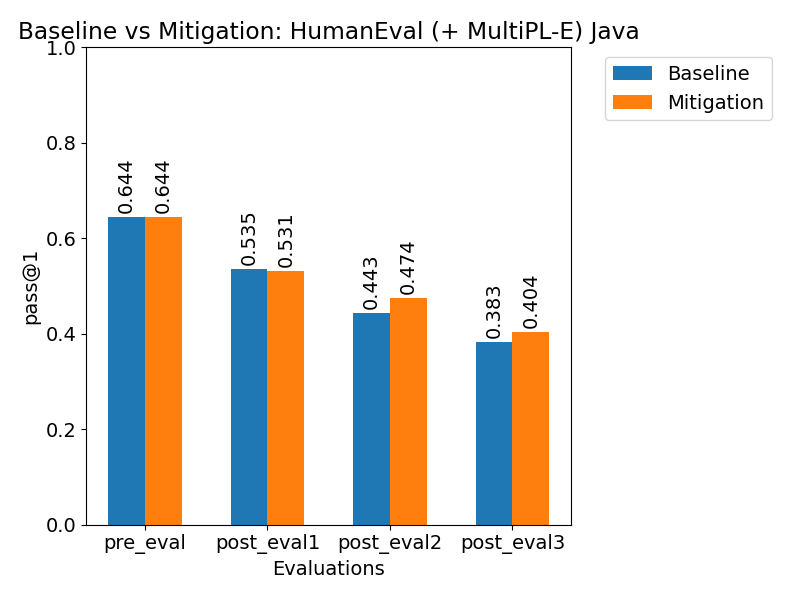
\includegraphics[width=0.8\textwidth]{Figures/results/code_comparisons/human_eval/comparison_humaneval_java.png} 
    \caption{Baseline vs. Mitigation for HumanEval (+ MultiPL-E) Java}
    \label{fig:JavaComparison}
\end{figure}
On comparing the results on the HumanEval (+ MultiPL-E) Java benchmark, we continued to observe the decline in performance across the post-evaluation stages. The addition of replay provided small improvements in post\_eval2 and post\_eval3.

\begin{figure}[H]
    \centering
    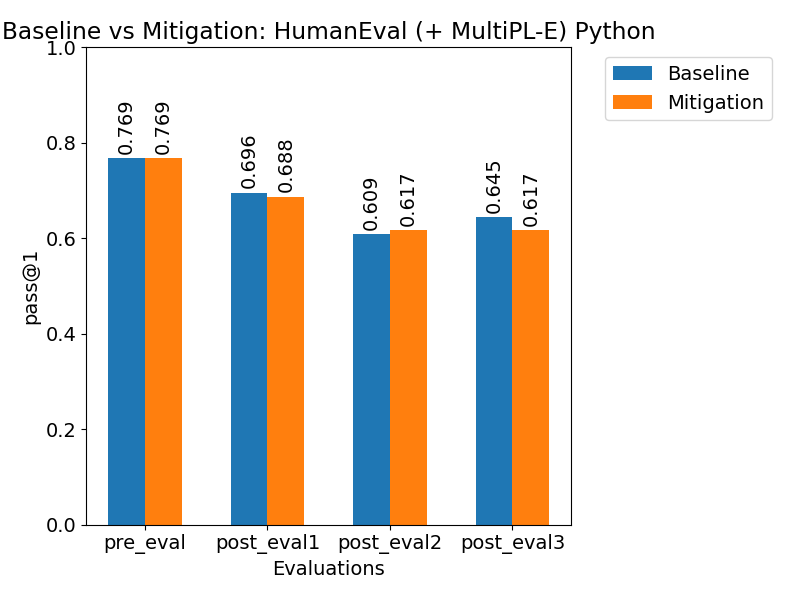
\includegraphics[width=0.8\textwidth]{Figures/results/code_comparisons/human_eval/comparison_humaneval_python.png} 
    \caption{Baseline vs. Mitigation for HumanEval (+ MultiPL-E) Python}
    \label{fig:PythonComparison}
\end{figure}
For the HumanEval (+ MultiPL-E) Python benchmark, there is an overall decline in the model performance, but the decline is not as severe compared to what was observed for Java and C++. However, the addition of replay mitigation degrades the performance more in comparison to the baseline runs.

\begin{figure}[H]
    \centering
    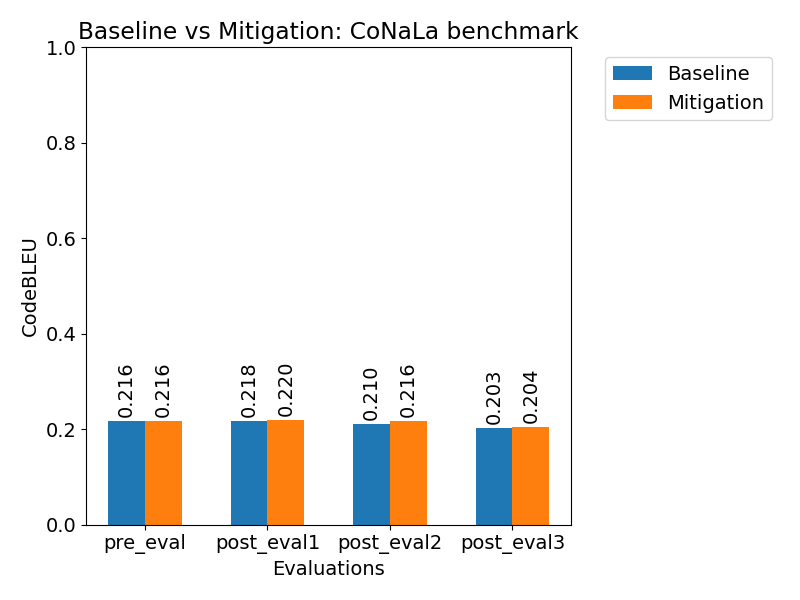
\includegraphics[width=0.8\textwidth]{Figures/results/code_comparisons/conala/comparison_conala.png} 
    \caption{Baseline vs. Mitigation for CoNaLa benchmark}
    \label{fig:ConalaComparison}
\end{figure}
For the CoNaLa benchmark, we observed that the performance remained stable across the post-evaluation stages. Additionally, the inclusion of replay mitigation did not make any impact on the performance on the CoNaLa benchmark.

\subsubsection{Impact on task-specific capabilities}
In this section, we compared the baseline and mitigation results on the task-specific evaluations.
\begin{figure}[H]
    \centering
    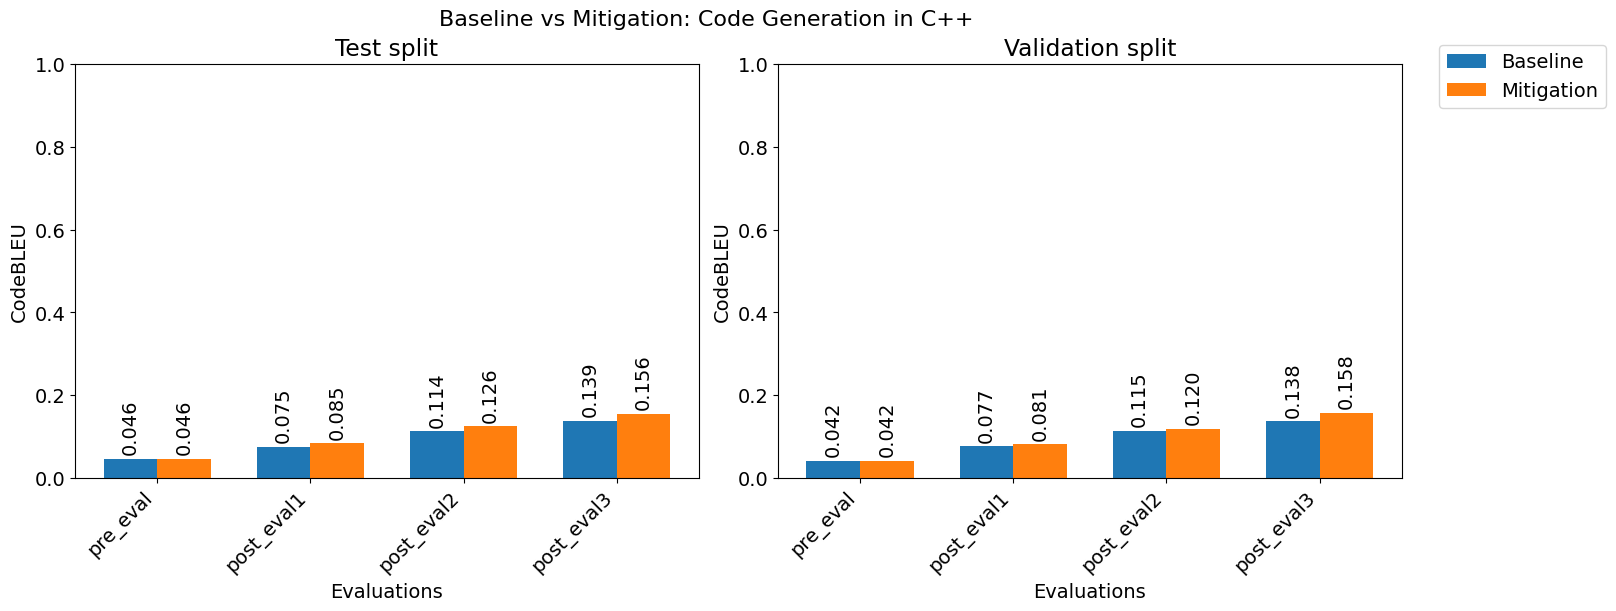
\includegraphics[width=1.2\textwidth]{Figures/results/code_comparisons/task_eval/comparison_task_cg.png} 
    \caption{Baseline vs. Mitigation for Code Generation in C++}
    \label{fig:CGComparison}
\end{figure}

% \begin{figure}[H]
%     \centering
%     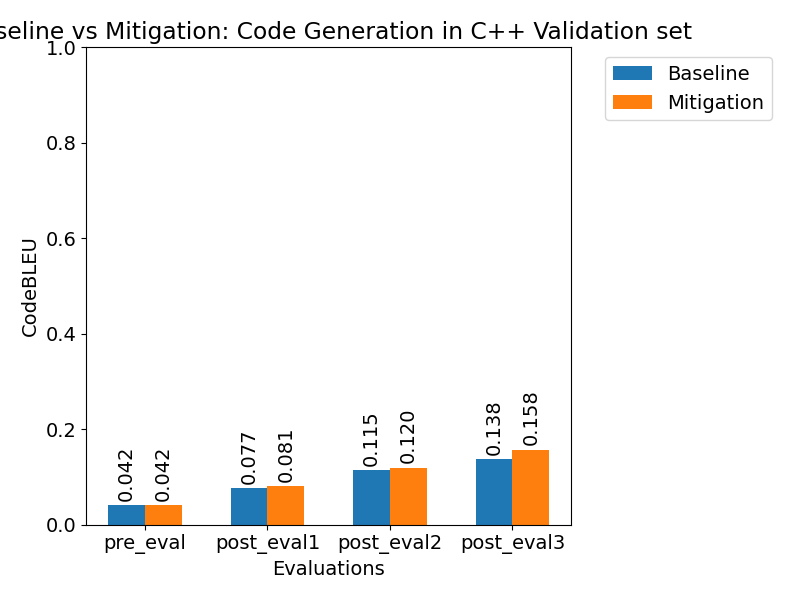
\includegraphics[width=0.8\textwidth]{Figures/results/code_comparisons/task_eval/comparison_task_cg_val.png} 
%     \caption{Baseline vs. Mitigation for Code Generation in C++ Validation set}
%     \label{fig:CGValComparison}
% \end{figure}
The comparison of the baseline and mitigation results on the cg task evaluation showed that for both runs, there was a continual improvement in the task performance across the post-evaluation stages. In post\_eval2 and post\_eval3, the mitigation run showed a very slight improvement over the baseline scores. However, we noted that for the task-specific evaluations, there is no degradation in performance and hence no forgetting. The inclusion of replay mitigation just served as more data for model training.

\begin{figure}[H]
    \centering
    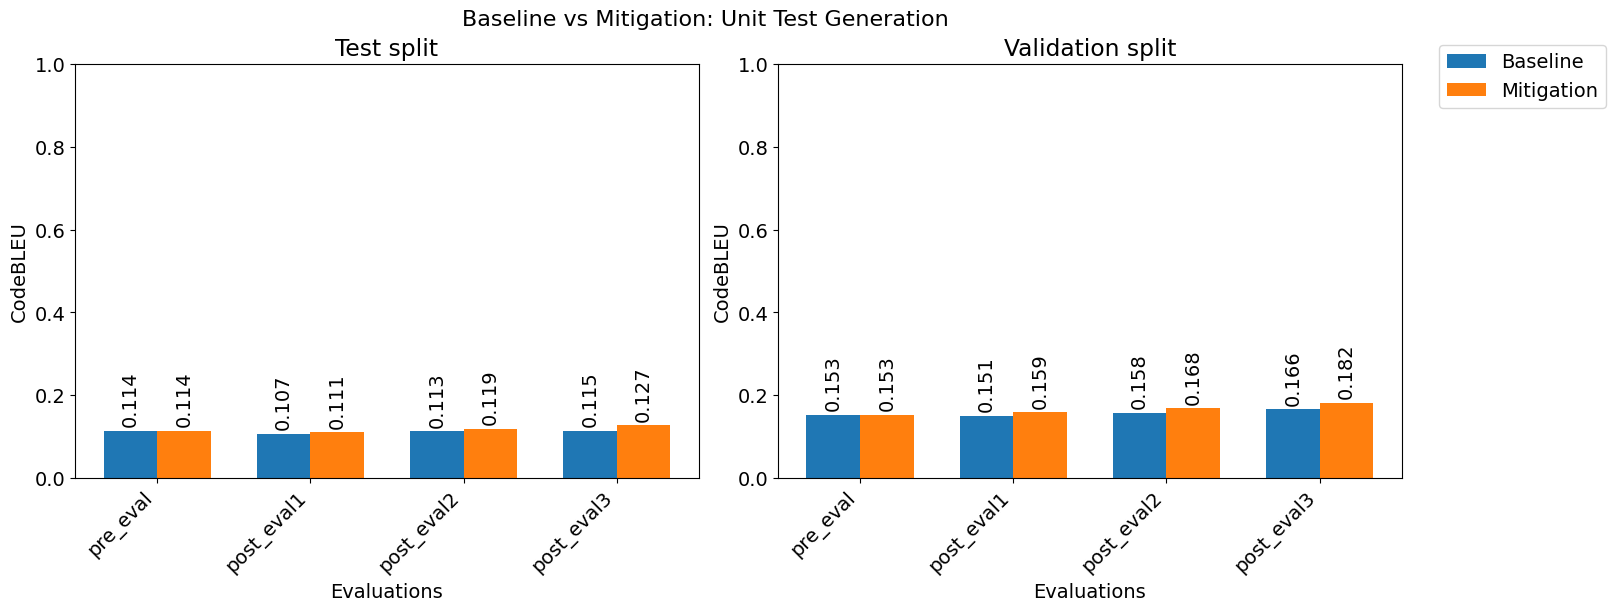
\includegraphics[width=1.2\textwidth]{Figures/results/code_comparisons/task_eval/comparison_task_utg.png} 
    \caption{Baseline vs. Mitigation for Unit Test Generation}
    \label{fig:UTGComparison}
\end{figure}

% \begin{figure}[H]
%     \centering
%     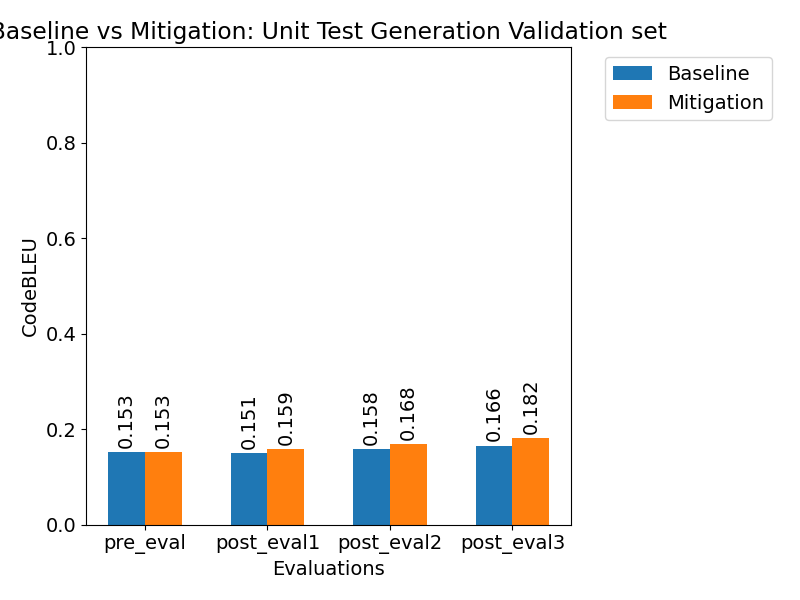
\includegraphics[width=1\textwidth]{Figures/results/code_comparisons/task_eval/comparison_task_utg_val.png}
%     \caption{Baseline vs. Mitigation for Unit Test Generation Validation set}
%     \label{fig:UTGValComparison}
% \end{figure}

On comparing the results of the utg task evaluation on both the test and validation sets, it was observed that the performance remained steady over the different post-evaluation stages, with the mitigation runs offering a tiny improvement over the baseline runs. 

\begin{figure}[H]
    \centering
    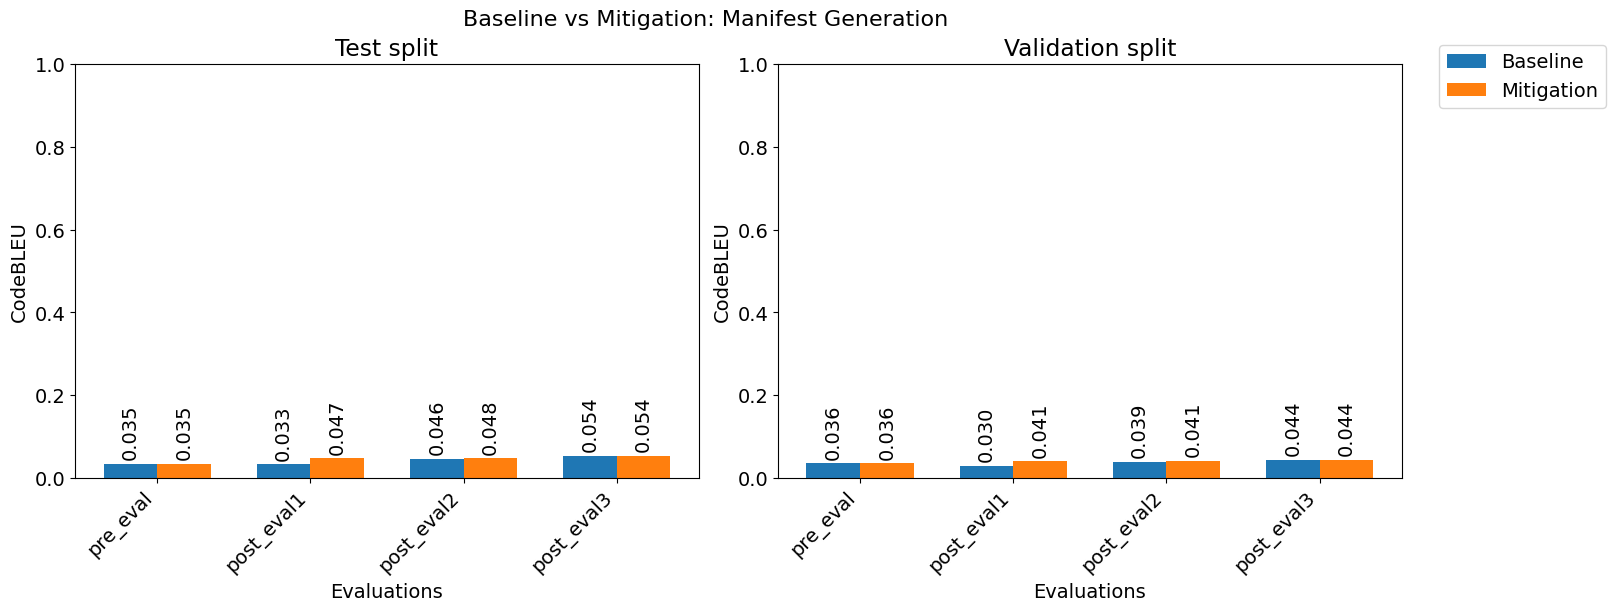
\includegraphics[width=1.2\textwidth]{Figures/results/code_comparisons/task_eval/comparison_task_mg.png} 
    \caption{Baseline vs. Mitigation for Manifest Generation}
    \label{fig:MGComparison}
\end{figure}

% \begin{figure}[H]
%     \centering
%     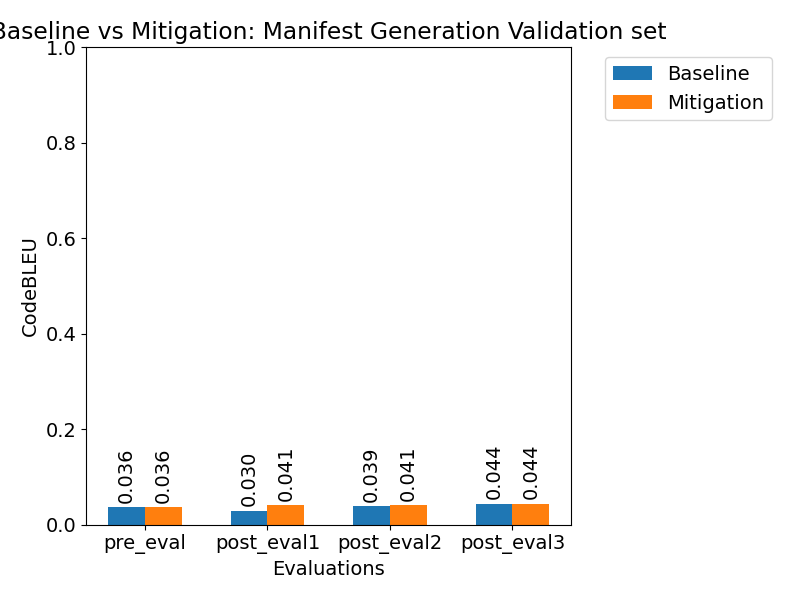
\includegraphics[width=1\textwidth]{Figures/results/code_comparisons/task_eval/comparison_task_mg_val.png} 
%     \caption{Baseline vs. Mitigation for Manifest Generation Validation set}
%     \label{fig:MGValComparison}
% \end{figure}

From the mg task evaluation results on the test and validation sets, it was observed that there was a tiny improvement in performance across the fine-tunes. Additionally, the inclusion of replay improves the performance slightly in post\_eval1. However, in the final post-evaluation stage, the baseline run slightly outperformed the mitigation run.

The comparison of the performance between the baseline and mitigation runs across the six different task sequences showed that the inclusion of replay mitigation step appeared to reduce the variance of the performance scores across task orders. To confirm this, we computed the standard deviation of the performance scores across the different ablations. The results from this study are presented in Tables \ref{tab:CodeBaselineStdDev} and \ref{tab:CodeMitigationStdDev}.
\begin{table}[H]
\centering
\caption{Standard Deviations across ablations: Baseline runs}
\begin{tabular}{|c|l|l|llll|}
\hline
\multirow{2}{*}{\textbf{Evaluation}}       & \multicolumn{1}{c|}{\multirow{2}{*}{\textbf{Dataset}}} & \multicolumn{1}{c|}{\multirow{2}{*}{\textbf{N}}} & \multicolumn{4}{c|}{Standard   Deviation}                                                                                                              \\ \cline{4-7} 
                                           & \multicolumn{1}{c|}{}                                  & \multicolumn{1}{c|}{}                            & \multicolumn{1}{l|}{\textbf{pre\_eval}} & \multicolumn{1}{l|}{\textbf{post\_eval1}} & \multicolumn{1}{l|}{\textbf{post\_eval2}} & \textbf{post\_eval3} \\ \hline
\multirow{3}{*}{HumanEval   (+ MultiPL-E)} & C++                                                    & 80                                               & \multicolumn{1}{l|}{0}                  & \multicolumn{1}{l|}{0.1078}               & \multicolumn{1}{l|}{0.0530}               & 0.0363               \\ \cline{2-7} 
                                           & Java                                                   & 80                                               & \multicolumn{1}{l|}{0}                  & \multicolumn{1}{l|}{0.0262}               & \multicolumn{1}{l|}{0.0781}               & 0.0826               \\ \cline{2-7} 
                                           & Python                                                 & 80                                               & \multicolumn{1}{l|}{0}                  & \multicolumn{1}{l|}{0.0206}               & \multicolumn{1}{l|}{0.0881}               & 0.0280               \\ \hline
CoNaLa                                     & CoNaLa                                                 & 100                                              & \multicolumn{1}{l|}{0}                  & \multicolumn{1}{l|}{0.0039}               & \multicolumn{1}{l|}{0.0067}               & 0.0027               \\ \hline
\multirow{2}{*}{cg}                        & Test                                                   & 500                                              & \multicolumn{1}{l|}{0}                  & \multicolumn{1}{l|}{0.0426}               & \multicolumn{1}{l|}{0.0393}               & 0.0078               \\ \cline{2-7} 
                                           & Validation                                             & 501                                              & \multicolumn{1}{l|}{0}                  & \multicolumn{1}{l|}{0.0468}               & \multicolumn{1}{l|}{0.0432}               & 0.0086               \\ \hline
\multirow{2}{*}{utg}                       & Test                                                   & 48                                               & \multicolumn{1}{l|}{0}                  & \multicolumn{1}{l|}{0.0163}               & \multicolumn{1}{l|}{0.0133}               & 0.0094               \\ \cline{2-7} 
                                           & Validation                                             & 48                                               & \multicolumn{1}{l|}{0}                  & \multicolumn{1}{l|}{0.0299}               & \multicolumn{1}{l|}{0.0199}               & 0.0097               \\ \hline
\multirow{2}{*}{mg}                        & Test                                                   & 145                                              & \multicolumn{1}{l|}{0}                  & \multicolumn{1}{l|}{0.0195}               & \multicolumn{1}{l|}{0.0117}               & 0.0027               \\ \cline{2-7} 
                                           & Validation                                             & 146                                              & \multicolumn{1}{l|}{0}                  & \multicolumn{1}{l|}{0.0159}               & \multicolumn{1}{l|}{0.0082}               & 0.0004               \\ \hline
\end{tabular}
\label{tab:CodeBaselineStdDev}
\end{table}

\begin{table}[H]
\centering
\caption{Standard Deviations across ablations: Mitigation runs}
\begin{tabular}{|c|l|l|llll|}
\hline
\multirow{2}{*}{\textbf{Evaluation}}       & \multicolumn{1}{c|}{\multirow{2}{*}{\textbf{Dataset}}} & \multicolumn{1}{c|}{\multirow{2}{*}{\textbf{N}}} & \multicolumn{4}{c|}{Standard   Deviation}                                                                                                              \\ \cline{4-7} 
                                           & \multicolumn{1}{c|}{}                                  & \multicolumn{1}{c|}{}                            & \multicolumn{1}{l|}{\textbf{pre\_eval}} & \multicolumn{1}{l|}{\textbf{post\_eval1}} & \multicolumn{1}{l|}{\textbf{post\_eval2}} & \textbf{post\_eval3} \\ \hline
\multirow{3}{*}{HumanEval   (+ MultiPL-E)} & C++                                                    & 80                                               & \multicolumn{1}{l|}{0}                  & \multicolumn{1}{l|}{0.0418}               & \multicolumn{1}{l|}{0.0389}               & 0.0318               \\ \cline{2-7} 
                                           & Java                                                   & 80                                               & \multicolumn{1}{l|}{0}                  & \multicolumn{1}{l|}{0.0619}               & \multicolumn{1}{l|}{0.0417}               & 0.0647               \\ \cline{2-7} 
                                           & Python                                                 & 80                                               & \multicolumn{1}{l|}{0}                  & \multicolumn{1}{l|}{0.0222}               & \multicolumn{1}{l|}{0.0471}               & 0.0358               \\ \hline
CoNaLa                                     & CoNaLa                                                 & 100                                              & \multicolumn{1}{l|}{0}                  & \multicolumn{1}{l|}{0.0028}               & \multicolumn{1}{l|}{0.0074}               & 0.0041               \\ \hline
\multirow{2}{*}{cg}                        & Test                                                   & 500                                              & \multicolumn{1}{l|}{0}                  & \multicolumn{1}{l|}{0.0416}               & \multicolumn{1}{l|}{0.0499}               & 0.0098               \\ \cline{2-7} 
                                           & Validation                                             & 501                                              & \multicolumn{1}{l|}{0}                  & \multicolumn{1}{l|}{0.0440}               & \multicolumn{1}{l|}{0.0487}               & 0.0065               \\ \hline
\multirow{2}{*}{utg}                       & Test                                                   & 48                                               & \multicolumn{1}{l|}{0}                  & \multicolumn{1}{l|}{0.0137}               & \multicolumn{1}{l|}{0.0131}               & 0.0060               \\ \cline{2-7} 
                                           & Validation                                             & 48                                               & \multicolumn{1}{l|}{0}                  & \multicolumn{1}{l|}{0.0220}               & \multicolumn{1}{l|}{0.0246}               & 0.0070               \\ \hline
\multirow{2}{*}{mg}                        & Test                                                   & 145                                              & \multicolumn{1}{l|}{0}                  & \multicolumn{1}{l|}{0.0050}               & \multicolumn{1}{l|}{0.0086}               & 0.0010               \\ \cline{2-7} 
                                           & Validation                                             & 146                                              & \multicolumn{1}{l|}{0}                  & \multicolumn{1}{l|}{0.0031}               & \multicolumn{1}{l|}{0.0051}               & 0.0008               \\ \hline
\end{tabular}
\label{tab:CodeMitigationStdDev}
\end{table}

The comparison of the standard deviations between the baseline and mitigation runs showed that the performance scores of the model across different task orders generally had less variance for the mitigation runs than for the baseline runs. 

\subsection{Impact of task order on forgetting} \label{CodeTaskOrderImpact}
To check the impact of task order on forgetting, we ablated the order  of tasks and conducted experiments with six different sequences of fine-tuning covering all permutations of the tasks. For Code Generation task, the sequences of tasks used is listed in Table \ref{tab:CodeTaskOrder}. This allowed us to study the impact of task order on the model's pre-trained and learned capabilities by comparing the performance of the model across the different task orders and thereby understand whether certain task orders are more effective at preserving the model's performance across the different benchmarks and task-specific evaluations. 

% \input{Chapters/ResultsSubpages/CodeTaskOrderExperiments}
\begin{figure}[H]
    \centering
    \begin{minipage}{0.45\textwidth}
        \centering
        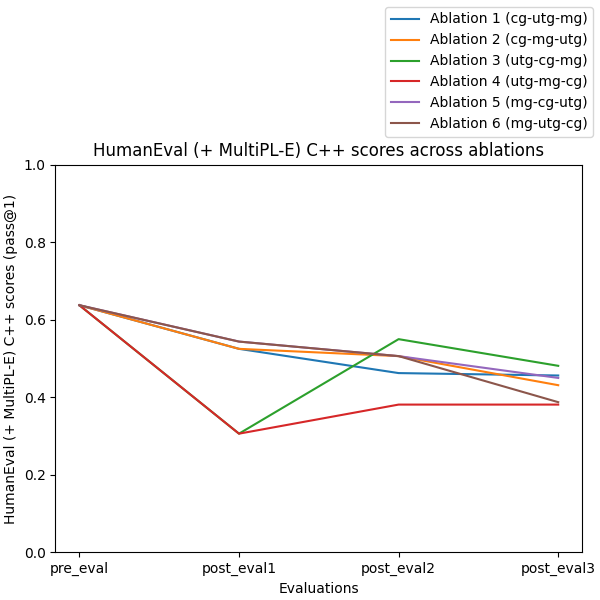
\includegraphics[width=1.1\textwidth]{Figures/results/code_baseline_graphs/human_eval/seed_averaged_humaneval_cpp_eval_baseline.png} % first figure itself
        \captionsetup{width=1.1\textwidth}
        \caption{HumanEval (+ MultiPL-E) C++: Baseline runs}
        \label{fig:CppAblationBaseline}
    \end{minipage}\hfill
    \begin{minipage}{0.45\textwidth}
        \centering
        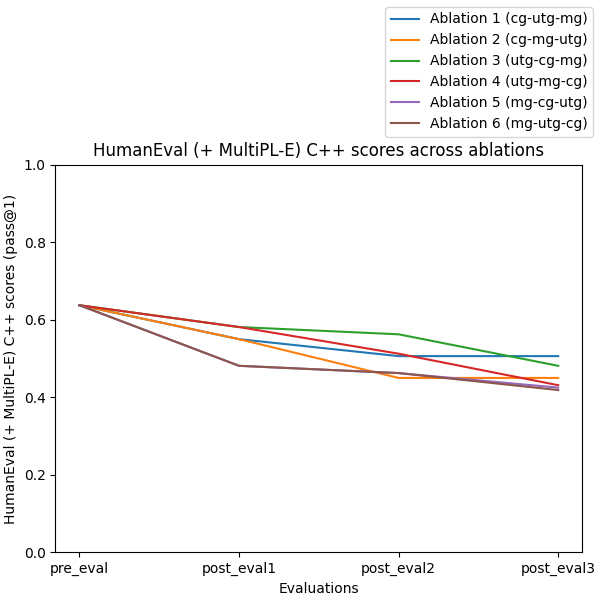
\includegraphics[width=1.1\textwidth]{Figures/results/code_mitigation_graphs/human_eval/seed_averaged_humaneval_cpp_eval_mitigation.png} % second figure itself
        \captionsetup{width=1.1\textwidth}
        \caption{HumanEval (+ MultiPL-E) C++: Mitigation runs}
        \label{fig:CppAblationMitigation}
    \end{minipage}
\end{figure}
The Figures \ref{fig:CppAblationBaseline} and \ref{fig:CppAblationMitigation} show the performance of the model on the HumanEval (+ MultiPL-E) C++ dataset for baseline and mitigation runs across the different ablations of task order sequences. From the charts, it was observed that different task sequences led to different results across the post-evaluation stages. The performance for different ablations appeared to have more variance in the baseline runs, and the mitigation runs were found to be more consistent across ablations. For the baseline runs, Ablation 4 (utg-mg-cg) had  the worst performance across all post-evaluation stages and Ablation 3 (utg-cg-mg) had dramatic performance drop and rise in post\_eval1 and post\_eval2 respectively. However, the performance differences between ablations were less pronounced in the mitigation runs. For both baseline and mitigation runs, the performance scores appeared to converge to similar scores at the final post-evaluation stage.

\begin{figure}[H]
    \centering
    \begin{minipage}{0.45\textwidth}
        \centering
        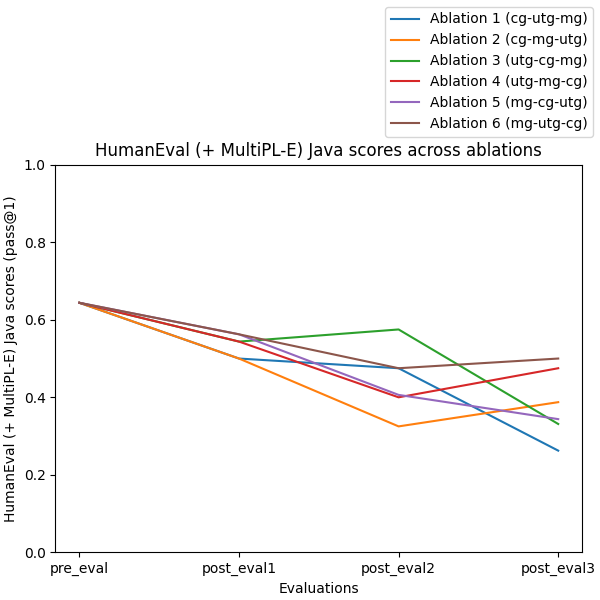
\includegraphics[width=1.1\textwidth]{Figures/results/code_baseline_graphs/human_eval/seed_averaged_humaneval_java_eval_baseline.png}
        \captionsetup{width=1.1\textwidth}
        \caption{HumanEval (+ MultiPL-E) Java: Baseline runs}
        \label{JavaBaselineAblations}
    \end{minipage}\hfill
    \begin{minipage}{0.45\textwidth}
        \centering
        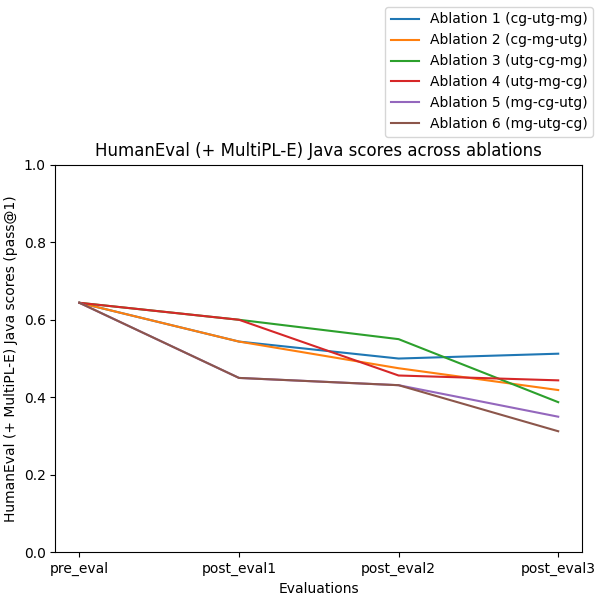
\includegraphics[width=1.1\textwidth]{Figures/results/code_mitigation_graphs/human_eval/seed_averaged_humaneval_java_eval_mitigation.png}
        \captionsetup{width=1.1\textwidth}
        \caption{HumanEval (+ MultiPL-E) Java: Mitigation runs}
        \label{JavaMitigationAblations}
    \end{minipage}
\end{figure}
From the performance of the model on HumanEval (+ MultiPL-E) Java benchmark (Figures: \ref{JavaBaselineAblations} and \ref{JavaMitigationAblations}) for the different ablations, we observed that the different ablations had a more variable performance on the final post-evaluation stage than for the C++ dataset. For instance: Ablation 1 (cg-utg-mg) and Ablation 6 (mg-utg-cg) had very different final performance scores in both baseline and mitigation runs, indicating that the order in which the tasks were fine-tuned affected the performance of the model. For the baseline runs, Ablation 1 (cg-utg-mg) and Ablation 3 (utg-cg-mg) showed initial drops for post\_eval1 with a small improvement in post\_eval2 before dropping again in post\_eval3. The mitigation runs showed more gradual declines across the ablations.

\begin{figure}[H]
    \centering
    \begin{minipage}{0.45\textwidth}
        \centering
        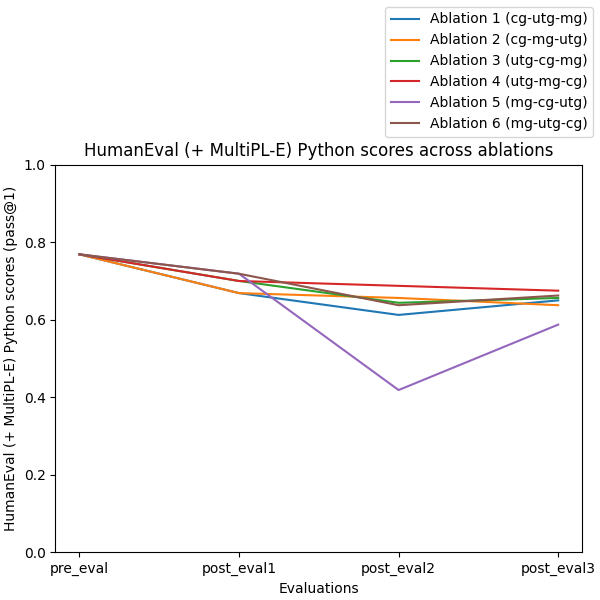
\includegraphics[width=1.1\textwidth]{Figures/results/code_baseline_graphs/human_eval/seed_averaged_humaneval_python_eval_baseline.png} % first figure itself
        \captionsetup{width=1.1\textwidth}
        \caption{HumanEval (+ MultiPL-E) Python: Baseline runs}
        \label{PythonBaselineAblations}
    \end{minipage}\hfill
    \begin{minipage}{0.45\textwidth}
        \centering
        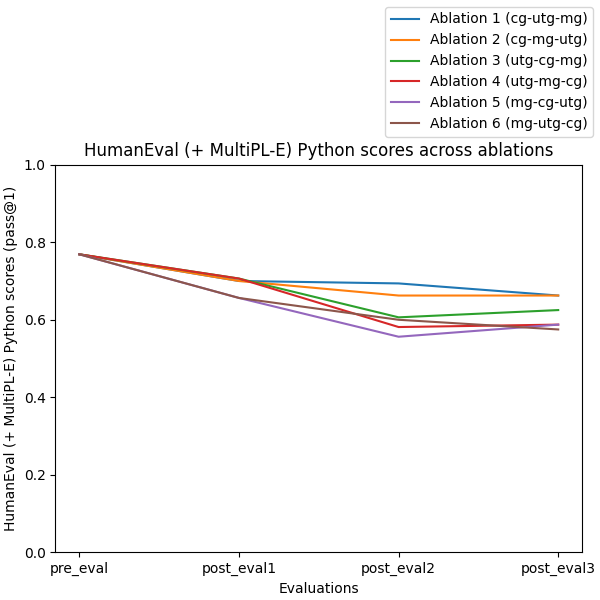
\includegraphics[width=1.1\textwidth]{Figures/results/code_mitigation_graphs/human_eval/seed_averaged_humaneval_python_eval_mitigation.png} % second figure itself
        \captionsetup{width=1.1\textwidth}
        \caption{HumanEval (+ MultiPL-E) Python: Mitigation runs}
        \label{PythonMitigationAblations}
    \end{minipage}
\end{figure}
From the comparison across ablations on the HumanEval (+ MultiPL-E) Python dataset (Figures: \ref{PythonBaselineAblations} and \ref{PythonMitigationAblations}), it was observed that the ablations had lesser variance in the baseline runs, except for Ablation 5 in post\_eval2. This showed that the performance on Python dataset did not vary much across ablations. However, for the mitigation runs, it can be observed that the ablations had more variance in post\_eval2 and post\_eval3.

\begin{figure}[H]
    \centering
    \begin{minipage}{0.45\textwidth}
        \centering
        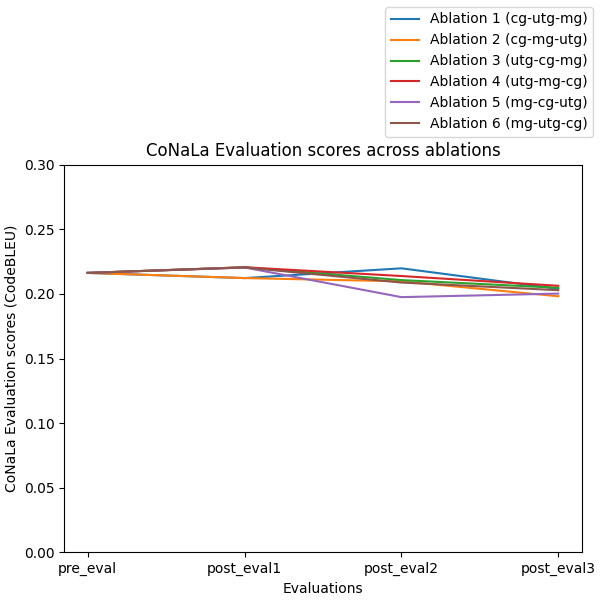
\includegraphics[width=1.1\textwidth]{Figures/results/code_baseline_graphs/conala/seed_averaged_conala_eval_baseline.png} % first figure itself
        \captionsetup{width=1.1\textwidth}
        \caption{CoNaLa benchmark: Baseline runs}
        \label{ConalaBaselineAblation}
    \end{minipage}\hfill
    \begin{minipage}{0.45\textwidth}
        \centering
        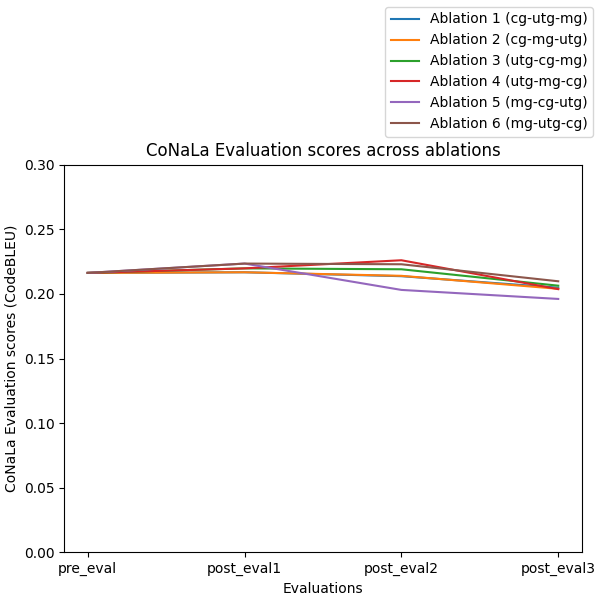
\includegraphics[width=1.1\textwidth]{Figures/results/code_mitigation_graphs/conala/seed_averaged_conala_eval_mitigation.png} % first figure itself
        \captionsetup{width=1.1\textwidth}
        \caption{CoNaLa benchmark: Mitigation runs}
        \label{ConalaMitigationAblation}
    \end{minipage}
\end{figure}
The performance of the model on the CoNaLa benchmark (Figures: \ref{ConalaBaselineAblation} and \ref{ConalaMitigationAblation}) remained relatively steady throughout all ablations for both baseline and mitigation runs.

\begin{figure}[H]
    \centering
    \begin{minipage}{0.45\textwidth}
        \centering
        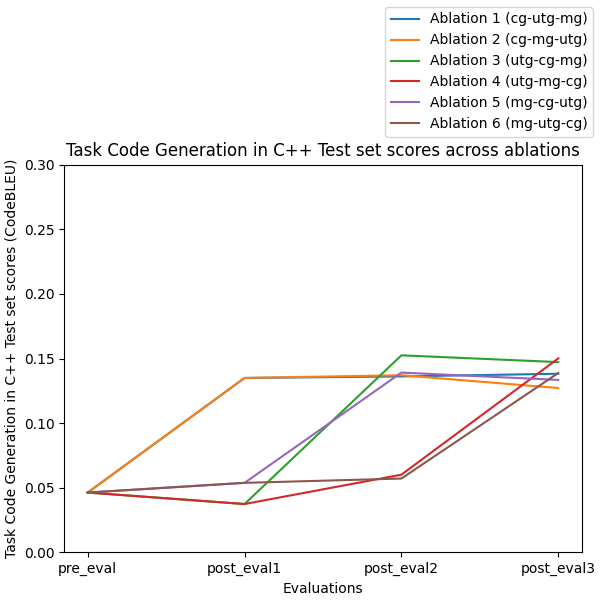
\includegraphics[width=1.1\textwidth]{Figures/results/code_baseline_graphs/task_eval/seed_averaged_task_cg_test_eval_baseline.png} % first figure itself
        \captionsetup{width=1.1\textwidth}
        \caption{Code Generation in C++ Test set: Baseline runs}
        \label{CGTestBaseline}
    \end{minipage}\hfill
    \begin{minipage}{0.45\textwidth}
        \centering
        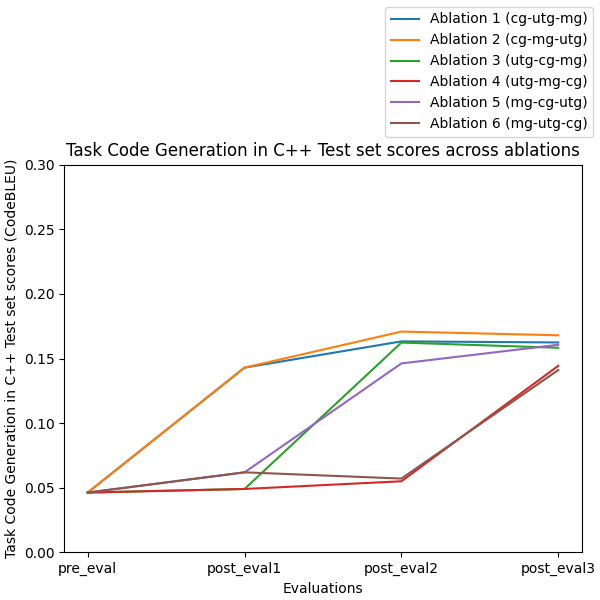
\includegraphics[width=1.1\textwidth]{Figures/results/code_mitigation_graphs/task_eval/seed_averaged_task_cg_test_eval_mitigation.png} % first figure itself
        \captionsetup{width=1.1\textwidth}
        \caption{Code Generation in C++ Test set: Mitigation runs}
        \label{CGTestMitigation}
    \end{minipage}
\end{figure}

\begin{figure}[H]
    \centering
    \begin{minipage}{0.45\textwidth}
        \centering
        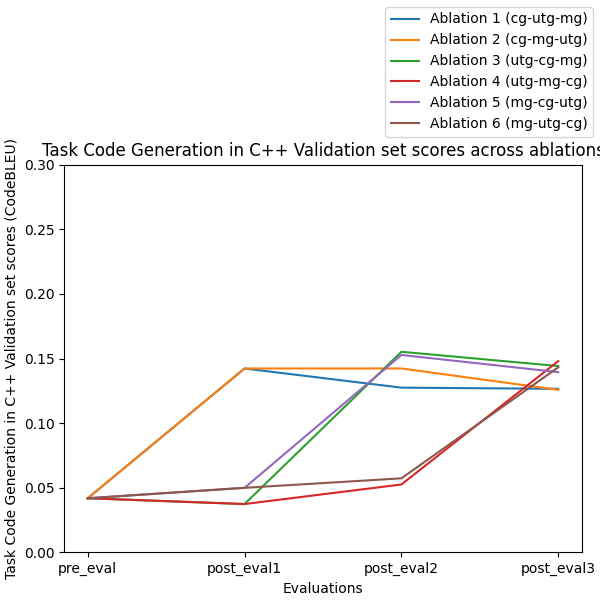
\includegraphics[width=1.1\textwidth]{Figures/results/code_baseline_graphs/task_eval/seed_averaged_task_cg_val_eval_baseline.png} % first figure itself
        \captionsetup{width=1.1\textwidth}
        \caption{Code Generation in C++ Validation set: Baseline runs}
        \label{CGValBaseline}
    \end{minipage}\hfill
    \begin{minipage}{0.45\textwidth}
        \centering
        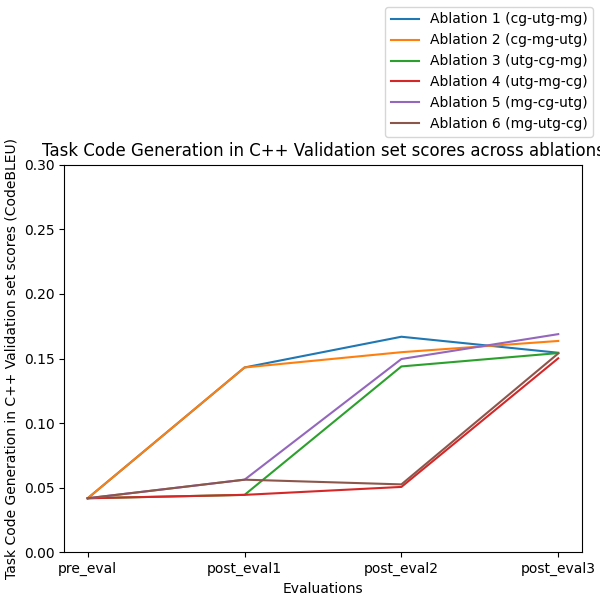
\includegraphics[width=1.1\textwidth]{Figures/results/code_mitigation_graphs/task_eval/seed_averaged_task_cg_val_eval_mitigation.png} % first figure itself
        \captionsetup{width=1.1\textwidth}
        \caption{Code Generation in C++ Validation set: Mitigation runs}
        \label{CGValMitigation}
    \end{minipage}
\end{figure}
The performance on the cg task (Figures: \ref{CGTestBaseline}, \ref{CGTestMitigation}, \ref{CGValBaseline} and \ref{CGValMitigation}) for the test and validation sets across the ablations showed greater variance in the scores for post\_eval1 and post\_eval2 for both baseline and mitigation runs. However, after the model had been trained on all tasks, the performance scores were less varied and seem to converge on post\_eval3. 

\begin{figure}[H]
    \centering
    \begin{minipage}{0.45\textwidth}
        \centering
        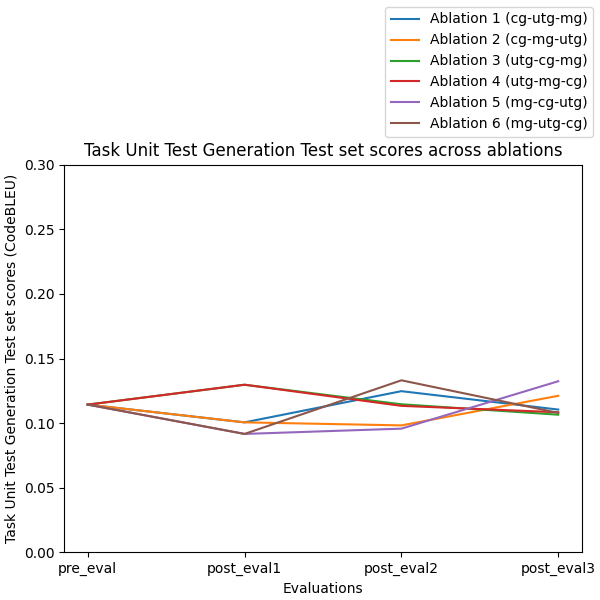
\includegraphics[width=1.1\textwidth]{Figures/results/code_baseline_graphs/task_eval/seed_averaged_task_utg_test_eval_baseline.png} % first figure itself
        \captionsetup{width=1.1\textwidth}
        \caption{Unit Test Generation Test set: Baseline runs}
        \label{UTGTestBaseline}
    \end{minipage}\hfill
    \begin{minipage}{0.45\textwidth}
        \centering
        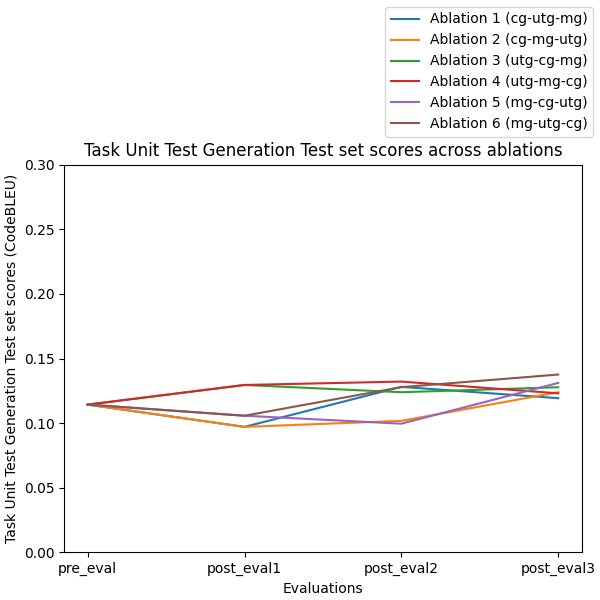
\includegraphics[width=1.1\textwidth]{Figures/results/code_mitigation_graphs/task_eval/seed_averaged_task_utg_test_eval_mitigation.png} % first figure itself
        \captionsetup{width=1.1\textwidth}
        \caption{Unit Test Generation Test set: Mitigation runs}
        \label{UTGTestMitigation}
    \end{minipage}
\end{figure}

\begin{figure}[H]
    \centering
    \begin{minipage}{0.45\textwidth}
        \centering
        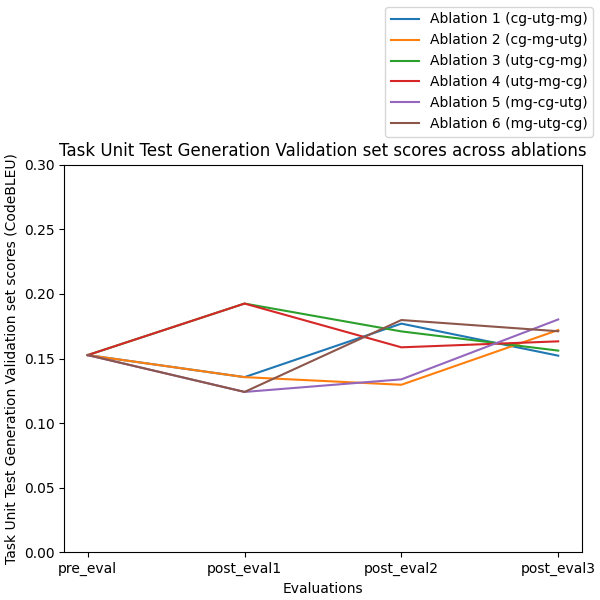
\includegraphics[width=1.1\textwidth]{Figures/results/code_baseline_graphs/task_eval/seed_averaged_task_utg_val_eval_baseline.png} % first figure itself
        \captionsetup{width=1.1\textwidth}
        \caption{Unit Test Generation Validation set: Baseline runs}
        \label{UTGValBaseline}
    \end{minipage}\hfill
    \begin{minipage}{0.45\textwidth}
        \centering
        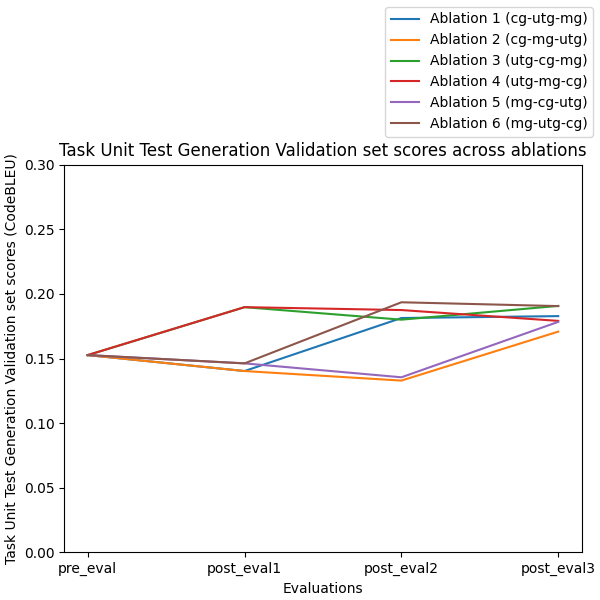
\includegraphics[width=1.1\textwidth]{Figures/results/code_mitigation_graphs/task_eval/seed_averaged_task_utg_val_eval_mitigation.png} % first figure itself
        \captionsetup{width=1.1\textwidth}
        \caption{Unit Test Generation Validation set: Mitigation runs}
        \label{UTGValMitigation}
    \end{minipage}
\end{figure}
For the utg task (Figures: \ref{UTGTestBaseline}, \ref{UTGTestMitigation}, \ref{UTGValBaseline} and \ref{UTGValMitigation}), it was observed that task order had more impact for the validation set than for the test set, with the test set having less variance in performance than the validation set. 

\begin{figure}[H]
    \centering
    \begin{minipage}{0.45\textwidth}
        \centering
        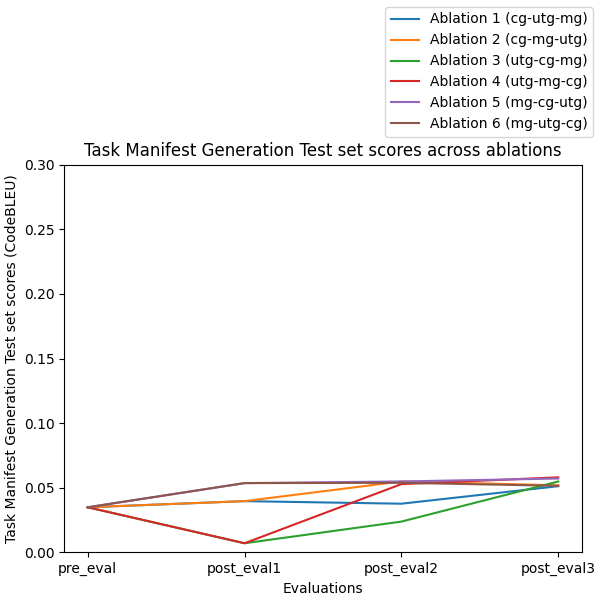
\includegraphics[width=1.1\textwidth]{Figures/results/code_baseline_graphs/task_eval/seed_averaged_task_mg_test_eval_baseline.png} % first figure itself
        \captionsetup{width=1.1\textwidth}
        \caption{Manifest Generation Test set: Baseline runs}
        \label{MGTestBaseline}
    \end{minipage}\hfill
    \begin{minipage}{0.45\textwidth}
        \centering
        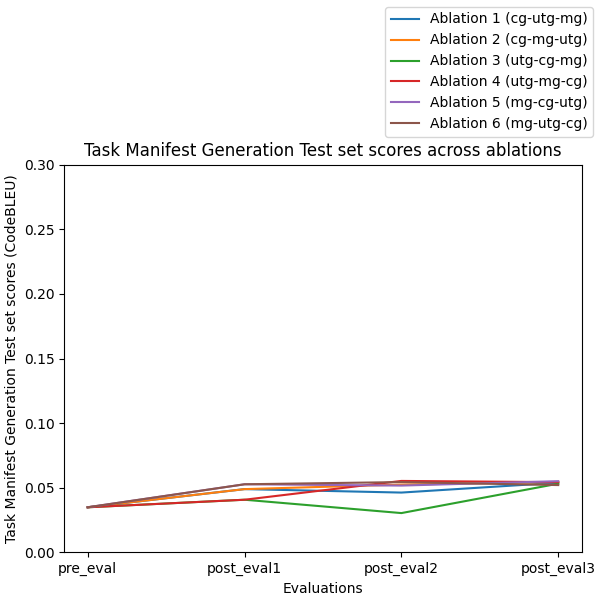
\includegraphics[width=1.1\textwidth]{Figures/results/code_mitigation_graphs/task_eval/seed_averaged_task_mg_test_eval_mitigation.png} % first figure itself
        \captionsetup{width=1.1\textwidth}
        \caption{Manifest Generation Test set: Mitigation runs}
        \label{MGTestMitigation}
    \end{minipage}
\end{figure}

\begin{figure}[H]
    \centering
    \begin{minipage}{0.45\textwidth}
        \centering
        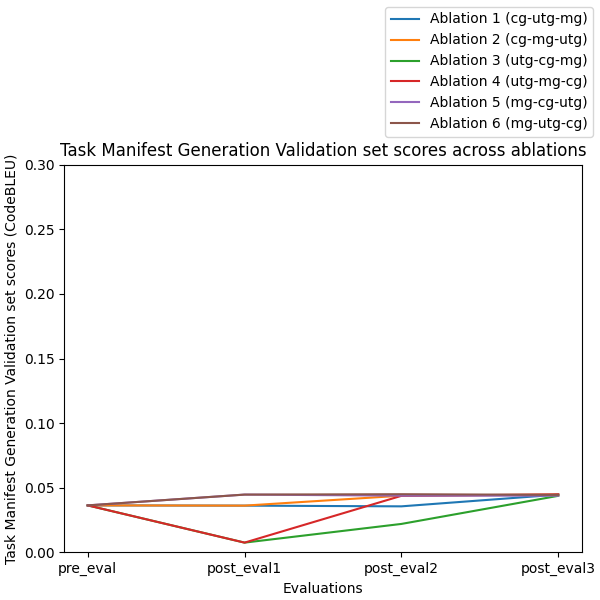
\includegraphics[width=1.1\textwidth]{Figures/results/code_baseline_graphs/task_eval/seed_averaged_task_mg_val_eval_baseline.png} % first figure itself
        \captionsetup{width=1.1\textwidth}
        \caption{Manifest Generation Validation set: Baseline runs}
        \label{MGValBaseline}
    \end{minipage}\hfill
    \begin{minipage}{0.45\textwidth}
        \centering
        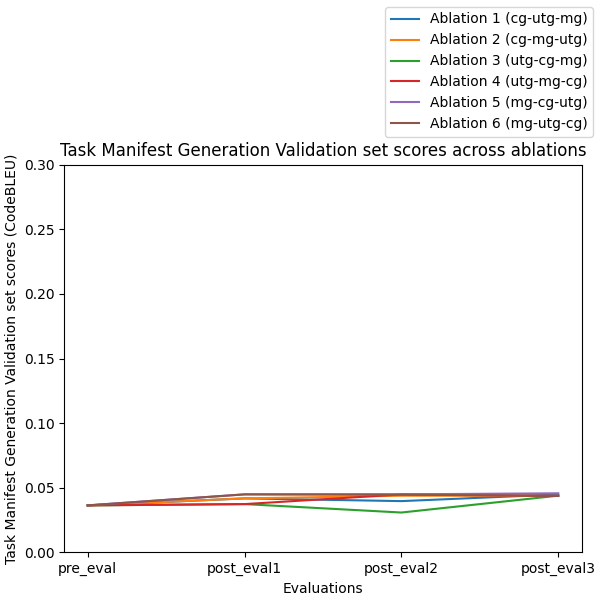
\includegraphics[width=1.1\textwidth]{Figures/results/code_mitigation_graphs/task_eval/seed_averaged_task_mg_val_eval_mitigation.png} % first figure itself
        \captionsetup{width=1.1\textwidth}
        \caption{Manifest Generation Validation set: Mitigation runs}
        \label{MGValMitigation}
    \end{minipage}
\end{figure}
For the mg task (Figures: \ref{MGTestBaseline}, \ref{MGTestMitigation}, \ref{MGValBaseline} and \ref{MGValMitigation}), it was observed that the final performance scores at post\_eval3 when the model has been trained on all three tasks are very similar. For the baseline runs, there are differences in the performances in post\_eval1 and post\_eval2, but the scores converge to similar values in the last post-evaluation stage. The mitigation runs were found to be very consistent across the ablations, showing the mitigation runs to have a more stable performance across the sequences with different orders of tasks.

\section{Natural Language Generation use case}
This section presents the results from the experiments carried out with Natural Language Generation use case tasks: Question Answering (qa), Summarization (summ), and Mathematical Reasoning (math).

\subsection{Evaluation of model's pre-trained capabilities}
Evaluation with different benchmarks and task-specific assessments have been conducted to measure and track the changes in the pre-trained capabilities of the instruct model across fine-tunes. In this section, the performance evaluation results of the Meta-Llama-3-8B-Instruct model on ARC-Challenge and GSM8K benchmarks and task-specific evaluations are presented in Table \ref{tab:TraceBenchmarkPreEval} and Table \ref{tab:TraceTaskEvalPreEval} respectively. These results have been obtained using a single seed value.

%----Table 1

\begin{table}[h!]
\centering
\caption{Performance of Meta-Llama-3-8B-Instruct on task-specific evaluations}
\begin{tabular}{lllll}
\hline
\multicolumn{1}{|l|}{Metric}                         & \multicolumn{1}{l|}{Evaluation   Benchmark} & \multicolumn{1}{l|}{Sample size (N)} & \multicolumn{1}{l|}{Score}  & \multicolumn{1}{l|}{Reported score} \\ \hline
\multicolumn{1}{|c|}{\multirow{2}{*}{Exact   Match}} & \multicolumn{1}{l|}{ARC-Challenge}          & \multicolumn{1}{l|}{1172}            & \multicolumn{1}{l|}{0.7594} & \multicolumn{1}{l|}{0.786}          \\ \cline{2-5} 
\multicolumn{1}{|c|}{}                               & \multicolumn{1}{l|}{GSM8K}                  & \multicolumn{1}{l|}{660}             & \multicolumn{1}{l|}{0.7909} & \multicolumn{1}{l|}{0.796}          \\ \hline
\label{tab:TraceBenchmarkPreEval}
\end{tabular}
\end{table}

\begin{table}[H]
\centering
\caption{Performance of Meta-Llama-3-8B-Instruct on task-specific evaluations}
\begin{tabular}{lllllll}
\cline{1-5}
\multicolumn{1}{|l|}{Task}                  & \multicolumn{1}{l|}{Metric}                       & \multicolumn{1}{l|}{Dataset}    & \multicolumn{1}{l|}{Sample Size (N)} & \multicolumn{1}{l|}{Score}  &  &  \\ \cline{1-5}
\multicolumn{1}{|c|}{\multirow{2}{*}{qa}}   & \multicolumn{1}{c|}{\multirow{2}{*}{Exact Match}} & \multicolumn{1}{l|}{Test}       & \multicolumn{1}{l|}{500}             & \multicolumn{1}{l|}{0.8260} &  &  \\ \cline{3-5}
\multicolumn{1}{|c|}{}                      & \multicolumn{1}{c|}{}                             & \multicolumn{1}{l|}{Validation} & \multicolumn{1}{l|}{500}             & \multicolumn{1}{l|}{0.7580} &  &  \\ \cline{1-5}
\multicolumn{1}{|c|}{\multirow{2}{*}{summ}} & \multicolumn{1}{c|}{\multirow{2}{*}{ROUGE-L}}     & \multicolumn{1}{l|}{Test}       & \multicolumn{1}{l|}{76}              & \multicolumn{1}{l|}{0.2943} &  &  \\ \cline{3-5}
\multicolumn{1}{|c|}{}                      & \multicolumn{1}{c|}{}                             & \multicolumn{1}{l|}{Validation} & \multicolumn{1}{l|}{77}              & \multicolumn{1}{l|}{0.2973} &  &  \\ \cline{1-5}
\multicolumn{1}{|c|}{\multirow{2}{*}{math}} & \multicolumn{1}{c|}{\multirow{2}{*}{Exact Match}} & \multicolumn{1}{l|}{Test}       & \multicolumn{1}{l|}{159}             & \multicolumn{1}{l|}{0.7296} &  &  \\ \cline{3-5}
\multicolumn{1}{|c|}{}                      & \multicolumn{1}{c|}{}                             & \multicolumn{1}{l|}{Validation} & \multicolumn{1}{l|}{160}             & \multicolumn{1}{l|}{0.7438} &  &  \\ \cline{1-5}
\end{tabular}
\label{tab:TraceTaskEvalPreEval}
\end{table}


The results from the benchmark evaluations showed that our evaluation results were relatively close to the reported scores for the ARC-Challenge and GSM8K benchmarks. 
The task-specific evaluation results showed that the instruct model Meta-Llama-3-8B-Instruct scored well on qa and math tasks, even before fine-tuning. The results on the qa test and validation datasets showed a performance difference of 0.07, which indicated a difference in the data distribution between the two sets. 

\subsection{Baseline experiment results}
% \begin{table}[h!]
% \centering
% \caption{Benchmarks and Task-specific evaluation results for Baseline runs of Natural Language Generation use case}
% \begin{tabular}{|l|l|S[table-format=2.4]|S[table-format=2.4]|S[table-format=2.4]|S[table-format=2.4]|}
% \hline
% \textbf{Evaluation} & \textbf{Dataset} & \textbf{pre\_eval} & \textbf{post\_eval1} & \textbf{post\_eval2} & \textbf{post\_eval3} \\ \hline
% ARC-Challenge & ARC-Challenge & 0.759385666 & 0.736916951 & 0.70847554 & 0.711035267 \\ \hline
% GSM8K & GSM8K & 0.790909091 & 0.765151515 & 0.762373737 & 0.751515152 \\ \hline
% \multirow{2}{*}{qa} & Test & 0.826 & 0.869333333 & 0.885 & 0.896 \\ \cline{2-6}
%                     & Validation & 0.758 & 0.821333333 & 0.842666667 & 0.857 \\ \hline
% \multirow{2}{*}{summ} & Test & 0.294261402 & 0.301425965 & 0.304687384 & 0.308262634 \\ \cline{2-6}
%                       & Validation & 0.297310372 & 0.304382296 & 0.307580755 & 0.311534812 \\ \hline
% \multirow{2}{*}{math} & Test & 0.729559748 & 0.742138365 & 0.676100629 & 0.705450734 \\ \cline{2-6}
%                       & Validation & 0.74375 & 0.7 & 0.666666667 & 0.70625 \\ \hline
% \end{tabular}
% \label{tab:TraceBaselineCombined}
% \end{table}

\begin{table}[H]
\centering
\caption{Benchmarks and Task-specific evaluation results for Baseline runs of Natural Language Generation use case}
\begin{tabular}{|c|l|l|l|l|l|l|}
\hline
\multicolumn{1}{|l|}{Evaluation} & Dataset       & N & pre\_eval & post\_eval1 & post\_eval2 & post\_eval3 \\ \hline
ARC-Challenge                    & ARC-Challenge & 1172            & 0.7594    & 0.7369      & 0.7085      & 0.7110      \\ \hline
GSM8K                            & GSM8K         & 660             & 0.7909    & 0.7652      & 0.7624      & 0.7515      \\ \hline
\multirow{2}{*}{qa}              & Test          & 500             & 0.8260    & 0.8693      & 0.8850      & 0.8960      \\ \cline{2-7} 
                                 & Validation    & 500             & 0.7580    & 0.8213      & 0.8427      & 0.8570      \\ \hline
\multirow{2}{*}{summ}            & Test          & 76              & 0.2943    & 0.3014      & 0.3047      & 0.3083      \\ \cline{2-7} 
                                 & Validation    & 77              & 0.2973    & 0.3044      & 0.3076      & 0.3115      \\ \hline
\multirow{2}{*}{math}            & Test          & 159             & 0.7296    & 0.7421      & 0.6761      & 0.7055      \\ \cline{2-7} 
                                 & Validation    & 160             & 0.7438    & 0.7000      & 0.6667      & 0.7063      \\ \hline
\end{tabular}
\label{tab:TraceBaselineCombined}
\end{table}

From the results of the Baseline experiments, it was observed that the performance scores of the model declined on the benchmark datasets over time. The decline in the performance of the benchmark datasets, although not as drastic as it was for the HumanEval (+ MultiPL-E) C++ and Java benchmarks for the Code Generation use case, were 0.05 and 0.04 for the ARC-Challenge and GSM8K benchmarks respectively from the pre-evaluation to the final post-evaluation assessment.  

On the task-specific evaluations, an improvement in the performance of qa task was observed across the post-evaluation stages for both the test and validation sets. For the summ task, the performance remained relatively steady across the post-evaluation stages. However, there was a decline in the performance on the math task in post-evaluations 1 and 2 with a small recovery in the final post-evaluation. The highest improvement in task performance was observed for the qa task, with a 0.07 gain in the test set and approximately 0.1 gain in the validation set. 

\subsection{Mitigation experiment results}
The results from the mitigation experiments on benchmark evaluations and task-specific performance evaluations are presented in Table \ref{tab:TraceMitigationCombined}. The presented results have been averaged across the results obtained for the six different fine-tuning sequences for task order (Table \ref{tab:GenTaskOrder}).
% \begin{table}[h!]
% \centering
% \caption{Benchmarks and Task-specific evaluation results for Mitigation runs of Natural Language Generation use case}
% \begin{tabular}{|l|l|S[table-format=2.4]|S[table-format=2.4]|S[table-format=2.4]|S[table-format=2.4]|}
% \hline
% \textbf{Evaluation} & \textbf{Dataset} & \textbf{pre\_eval} & \textbf{post\_eval1} & \textbf{post\_eval2} & \textbf{post\_eval3} \\ \hline
% ARC-Challenge & ARC-Challenge & 0.759385666 & 0.74374289 & 0.734641638 & 0.711035267 \\ \hline
% GSM8K & GSM8K & 0.790909091 & 0.792929293 & 0.784848485 & 0.772979798 \\ \hline
% \multirow{2}{*}{qa} & Test & 0.826 & 0.886666667 & 0.892333333 & 0.829 \\ \cline{2-6}
%                     & Validation & 0.758 & 0.835333333 & 0.860333333 & 0.798666667 \\ \hline
% \multirow{2}{*}{summ} & Test & 0.294261402 & 0.299930822 & 0.303906716 & 0.306643941 \\ \cline{2-6}
%                       & Validation & 0.297310372 & 0.300932689 & 0.305942176 & 0.307397246 \\ \hline
% \multirow{2}{*}{math} & Test & 0.729559748 & 0.758909853 & 0.747379455 & 0.69706499 \\ \cline{2-6}
%                       & Validation & 0.74375 & 0.735416667 & 0.75 & 0.738541667 \\ \hline
% \end{tabular}
% \label{tab:TraceMitigationCombined}
% \end{table}

\begin{table}[H]
\centering
\caption{Benchmarks and Task-specific evaluation results for Mitigation runs of Natural Language Generation use case}
\begin{tabular}{|c|l|l|l|l|l|l|}
\hline
\multicolumn{1}{|l|}{Evaluation} & Dataset       & N & pre\_eval & post\_eval1 & post\_eval2 & post\_eval3 \\ \hline
ARC-Challenge                    & ARC-Challenge & 1172            & 0.7594    & 0.7437      & 0.7346      & 0.7110      \\ \hline
GSM8K                            & GSM8K         & 660             & 0.7909    & 0.7929      & 0.7848      & 0.7730      \\ \hline
\multirow{2}{*}{qa}              & Test          & 500             & 0.8260    & 0.8867      & 0.8923      & 0.8290      \\ \cline{2-7} 
                                 & Validation    & 500             & 0.7580    & 0.8353      & 0.8603      & 0.7987      \\ \hline
\multirow{2}{*}{summ}            & Test          & 76              & 0.2943    & 0.2999      & 0.3039      & 0.3066      \\ \cline{2-7} 
                                 & Validation    & 77              & 0.2973    & 0.3009      & 0.3059      & 0.3074      \\ \hline
\multirow{2}{*}{math}            & Test          & 159             & 0.7296    & 0.7589      & 0.7474      & 0.6971      \\ \cline{2-7} 
                                 & Validation    & 160             & 0.7438    & 0.7354      & 0.7500      & 0.7385      \\ \hline
\end{tabular}
\label{tab:TraceMitigationCombined}
\end{table}

The mitigation results showed that there was still a decline in the model's performance on the benchmarks, even with the addition of replay-based mitigation. 

An improvement in the performance scores for the qa task was observed for post\_eval1 and post\_eval2. However, there was a decline in performance for both the test and validation sets after the model was trained on the third task. This could indicate forgetting of task-specific capabilities across fine-tunes. For the summ task, the performance remained steady across all post-evaluation stages. The results were mixed for the math task with the test set performance showing a small improvement in post\_eval1, which declined in post\_eval2 and post\_eval3. For the validation set, the performance was noted to be unsteady across the post-evaluation stages.

\subsection{Baseline vs. Mitigation performance}
To measure the impact of the addition of replay mitigation, we compared the performance in the baseline results with the mitigation results.

\subsubsection{Impact on pre-trained model capabilities}
The comparisons between baseline and mitigation runs for Natural Language Generation use case on the benchmark datasets are presented in Figures \ref{fig:ArcComparison} and \ref{fig:GSM8kComparison}. 
\begin{figure}[H]
    \centering
    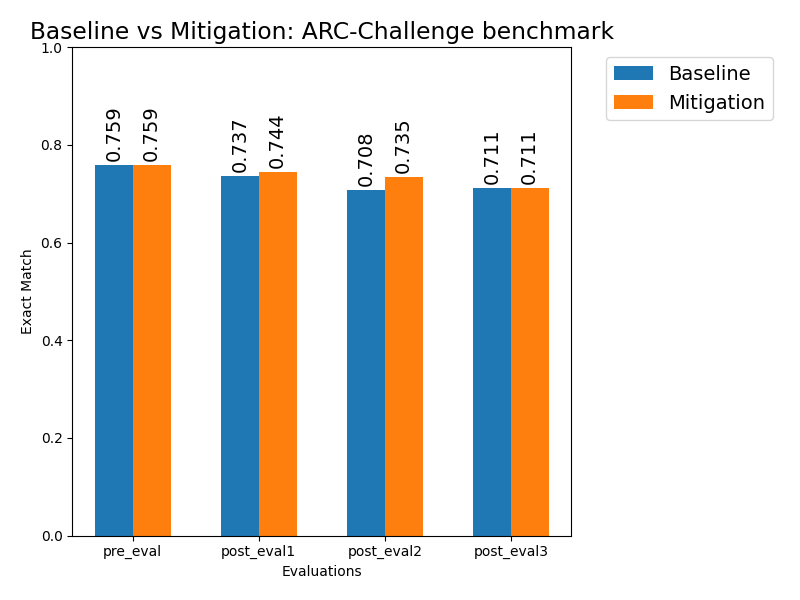
\includegraphics[width=0.8\textwidth]{Figures/results/trace_comparisons/arc_challenge/comparison_arc_challenge.png} 
    \caption{Baseline vs. Mitigation for ARC-Challenge Benchmark}
    \label{fig:ArcComparison}
\end{figure}
The comparison of the baseline and mitigation results on the ARC-Challenge benchmark showed that there was a decline in the performance scores for both runs across the evaluation stages. The addition of replay mitigation provided a slight boost in scores in post\_eval1 and post\_eval2 in comparison to the baseline run. However, in the final post-evaluation stage, both runs yielded the same score.

\begin{figure}[H]
    \centering
    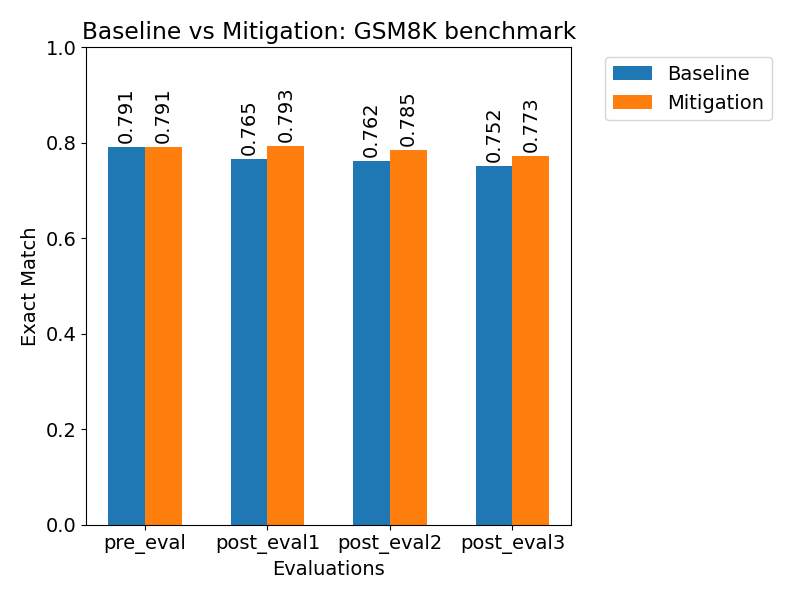
\includegraphics[width=0.8\textwidth]{Figures/results/trace_comparisons/gsm8k/comparison_gsm8k.png} 
    \caption{Baseline vs. Mitigation for GSM8K Benchmark}
    \label{fig:GSM8kComparison}
\end{figure}
For the GSM8K benchmark, we continued to see the performance decline trend for both baseline and mitigation runs. However, the addition of replay mitigation provided a slight improvement over the baseline scores across all post-evaluation stages.

\subsubsection{Impact on task-specific capabilities}
In this section, we compared the baseline and mitigation results on the task-specific evaluations.
\begin{figure}[H]
    \centering
    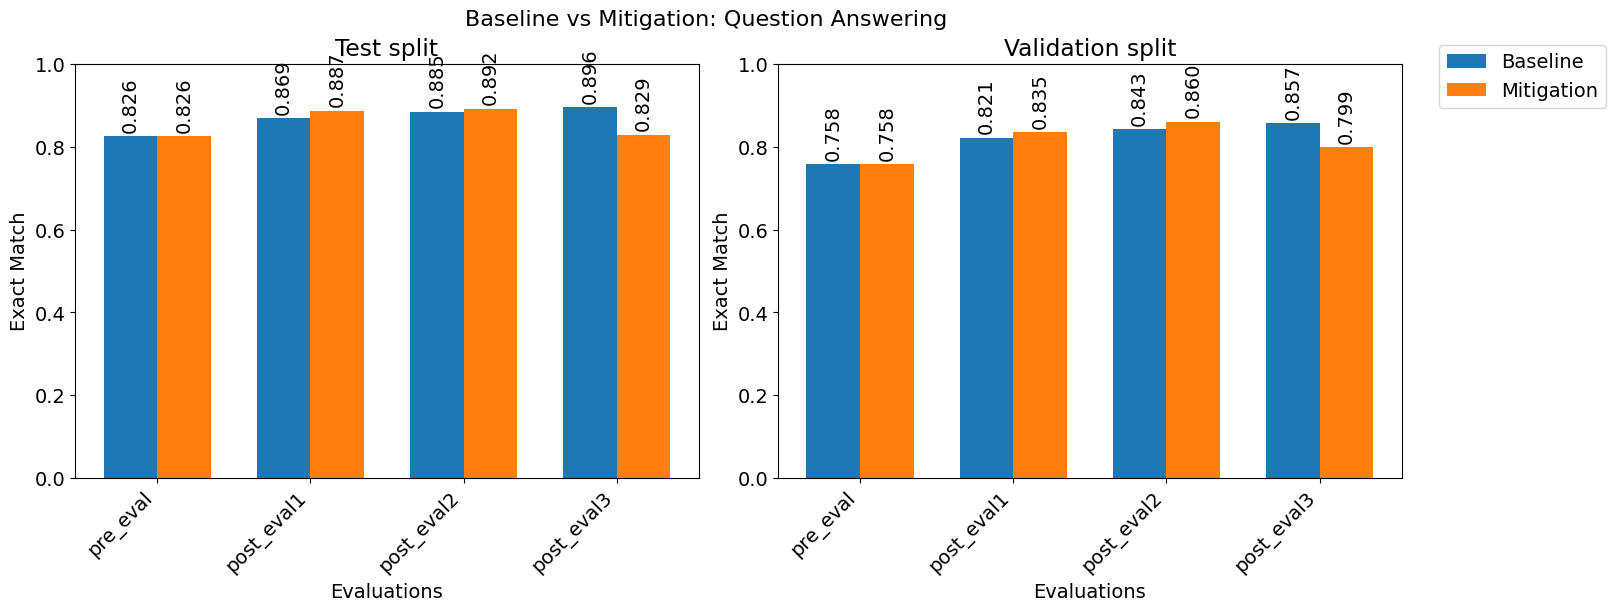
\includegraphics[width=1.1\textwidth]{Figures/results/trace_comparisons/task_eval/comparison_task_qa.png} 
    \caption{Baseline vs. Mitigation: Question Answering (qa)}
    \label{fig:QAComparison}
\end{figure}
The comparison of baseline and mitigation results on the qa task showed that the addition of replay mitigation provided a tiny boost in performance in post\_eval1 and post\_eval2. However, the performance in the final post-evaluation stage for the mitigation run suffered a substantial drop, resulting in the baseline run outperforming the mitigation run for qa task.

\begin{figure}[H]
    \centering
    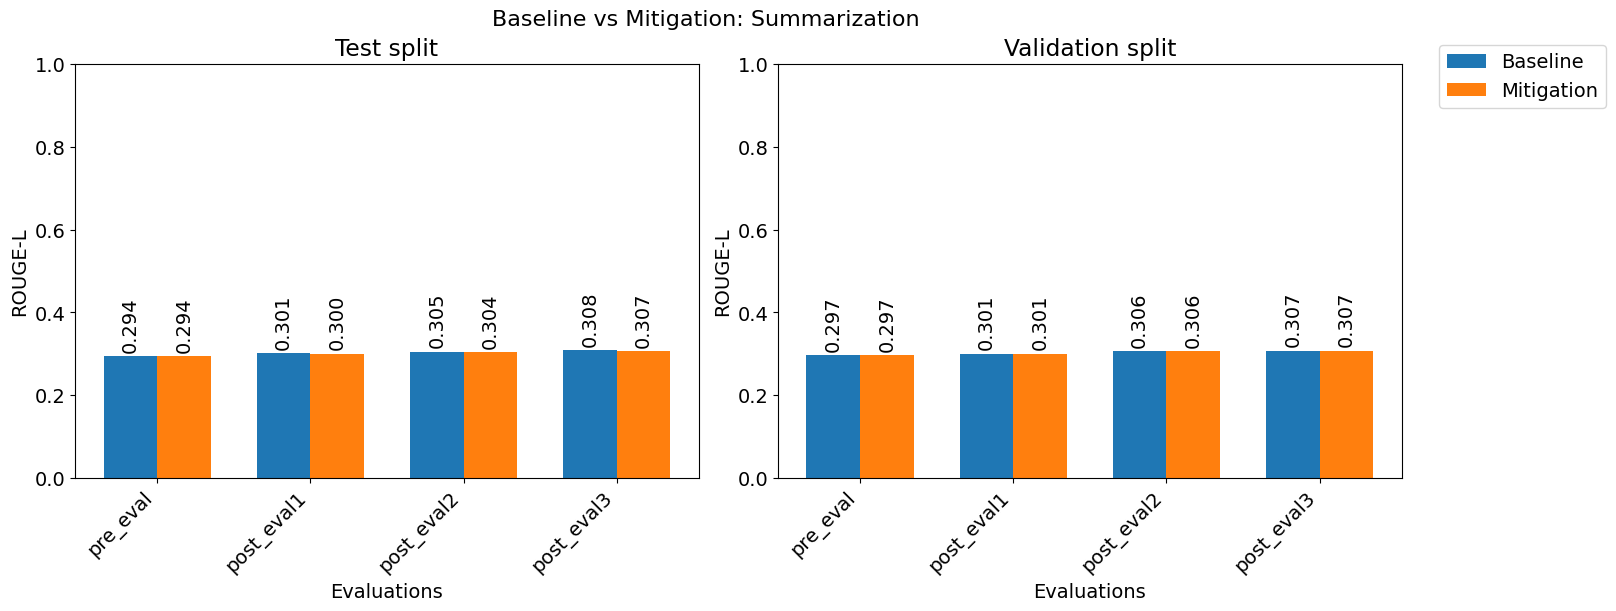
\includegraphics[width=1.1\textwidth]{Figures/results/trace_comparisons/task_eval/comparison_task_summ.png} 
    \caption{Baseline vs. Mitigation: Summarization (summ)}
    \label{fig:SummComparison}
\end{figure}
The performance on the summ task remained steady for both the baseline and mitigation runs throughout the post-evaluation stages.

\begin{figure}[H]
    \centering
    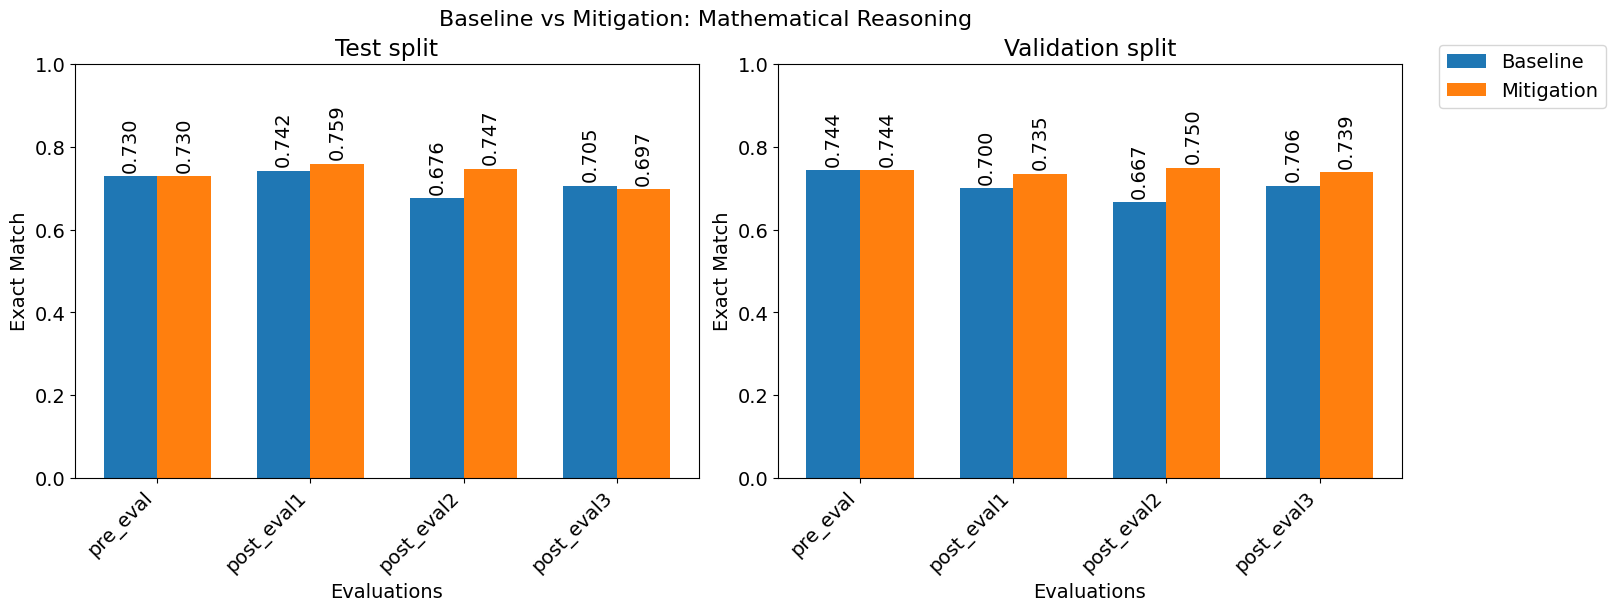
\includegraphics[width=1.1\textwidth]{Figures/results/trace_comparisons/task_eval/comparison_task_math.png} 
    \caption{Baseline vs. Mitigation: Mathematical Reasoning (math)}
    \label{fig:MathTestComparison}
\end{figure}
The comparison of the performance on the math task between the baseline and mitigation runs showed that there was a decline in performance for both runs. For the test set, there was an initial improvement in scores for both the runs in post\_eval1. However, this was followed by a decline in post\_eval2 and post\_eval3 for the mitigation run and a considerable decline followed by a small recovery for the baseline run. For the validation set, we observed a different trend, where the performance on the baseline run declined in post\_eval1 and post\_eval2 followed by a small recovery in post\_eval3. The performance on the mitigation run was more stable compared to the baseline run, with the decline in performance being smaller than that for the baseline run.

Similar to what was observed for the Code Generation use case, the comparison between the baseline and mitigation runs showed that the addition of replay mitigation appeared to reduce the variance in performance scores across the different sequences of the task order. To confirm this, we computed the standard deviations for the performance scores across the different sequences for both baseline and mitigation runs.   

\begin{table}[H]
\caption{Standard deviations across task order ablations: Baseline}
\begin{tabular}{|c|l|l|llll|}
\hline
\multirow{2}{*}{Evaluation} & \multicolumn{1}{c|}{\multirow{2}{*}{Dataset}} & \multicolumn{1}{c|}{\multirow{2}{*}{N}} & \multicolumn{4}{c|}{Standard   Deviation}                                                                          \\ \cline{4-7} 
                            & \multicolumn{1}{c|}{}                         & \multicolumn{1}{c|}{}                   & \multicolumn{1}{l|}{pre\_eval} & \multicolumn{1}{l|}{post\_eval1} & \multicolumn{1}{l|}{post\_eval2} & post\_eval3 \\ \hline
ARC-Challenge               & ARC-Challenge                                 & 1172                                    & \multicolumn{1}{l|}{0}         & \multicolumn{1}{l|}{0.0323}      & \multicolumn{1}{l|}{0.0608}      & 0.0267      \\ \hline
GSM8K                       & GSM8K                                         & 660                                     & \multicolumn{1}{l|}{0}         & \multicolumn{1}{l|}{0.0155}      & \multicolumn{1}{l|}{0.0228}      & 0.0166      \\ \hline
\multirow{2}{*}{qa}         & Test                                          & 500                                     & \multicolumn{1}{l|}{0}         & \multicolumn{1}{l|}{0.0340}      & \multicolumn{1}{l|}{0.0161}      & 0.0135      \\ \cline{2-7} 
                            & Validation                                    & 500                                     & \multicolumn{1}{l|}{0}         & \multicolumn{1}{l|}{0.0467}      & \multicolumn{1}{l|}{0.0196}      & 0.0181      \\ \hline
\multirow{2}{*}{summ}       & Test                                          & 76                                      & \multicolumn{1}{l|}{0}         & \multicolumn{1}{l|}{0.0074}      & \multicolumn{1}{l|}{0.0097}      & 0.0019      \\ \cline{2-7} 
                            & Validation                                    & 77                                      & \multicolumn{1}{l|}{0}         & \multicolumn{1}{l|}{0.0076}      & \multicolumn{1}{l|}{0.0079}      & 0.0026      \\ \hline
\multirow{2}{*}{math}       & Test                                          & 159                                     & \multicolumn{1}{l|}{0}         & \multicolumn{1}{l|}{0.0308}      & \multicolumn{1}{l|}{0.1077}      & 0.0534      \\ \cline{2-7} 
                            & Validation                                    & 160                                     & \multicolumn{1}{l|}{0}         & \multicolumn{1}{l|}{0.0736}      & \multicolumn{1}{l|}{0.1129}      & 0.0415      \\ \hline
\end{tabular}
\label{TraceBaselineStdDev}
\end{table}

\begin{table}[H]
\caption{Standard deviations across task order ablations: Mitigation}
\begin{tabular}{|c|l|l|llll|}
\hline
\multirow{2}{*}{Evaluation} & \multicolumn{1}{c|}{\multirow{2}{*}{Dataset}} & \multicolumn{1}{c|}{\multirow{2}{*}{N}} & \multicolumn{4}{c|}{Standard   Deviation}                                                                          \\ \cline{4-7} 
                            & \multicolumn{1}{c|}{}                         & \multicolumn{1}{c|}{}                                 & \multicolumn{1}{l|}{pre\_eval} & \multicolumn{1}{l|}{post\_eval1} & \multicolumn{1}{l|}{post\_eval2} & post\_eval3 \\ \hline
ARC-Challenge               & ARC-Challenge                                 & 1172                                                  & \multicolumn{1}{l|}{0}         & \multicolumn{1}{l|}{0.0251}      & \multicolumn{1}{l|}{0.0254}      & 0.0177      \\ \hline
GSM8K                       & GSM8K                                         & 660                                                   & \multicolumn{1}{l|}{0}         & \multicolumn{1}{l|}{0.0056}      & \multicolumn{1}{l|}{0.0113}      & 0.0093      \\ \hline
\multirow{2}{*}{qa}         & Test                                          & 500                                                   & \multicolumn{1}{l|}{0}         & \multicolumn{1}{l|}{0.0189}      & \multicolumn{1}{l|}{0.0078}      & 0.0466      \\ \cline{2-7} 
                            & Validation                                    & 500                                                   & \multicolumn{1}{l|}{0}         & \multicolumn{1}{l|}{0.0082}      & \multicolumn{1}{l|}{0.0076}      & 0.0160      \\ \hline
\multirow{2}{*}{summ}       & Test                                          & 76                                                    & \multicolumn{1}{l|}{0}         & \multicolumn{1}{l|}{0.0094}      & \multicolumn{1}{l|}{0.0091}      & 0.0041      \\ \cline{2-7} 
                            & Validation                                    & 77                                                    & \multicolumn{1}{l|}{0}         & \multicolumn{1}{l|}{0.0098}      & \multicolumn{1}{l|}{0.0084}      & 0.0040      \\ \hline
\multirow{2}{*}{math}       & Test                                          & 159                                                   & \multicolumn{1}{l|}{0}         & \multicolumn{1}{l|}{0.0292}      & \multicolumn{1}{l|}{0.0562}      & 0.0255      \\ \cline{2-7} 
                            & Validation                                    & 160                                                   & \multicolumn{1}{l|}{0}         & \multicolumn{1}{l|}{0.0463}      & \multicolumn{1}{l|}{0.0325}      & 0.0322      \\ \hline
\end{tabular}
\label{TraceMitigationStdDev}
\end{table}

From the above tables, it was observed that the standard deviation scores for both benchmarks were lower in all the post-evaluation stages of the mitigation run. For the task-specific evaluations, the standard deviations were found to be lower for post\_eval1 and post\_eval2 for qa task in the mitigation run. However, the variance in post\_eval3 was found to be greater for the mitigation run than for the baseline run for qa task. For the summ task, the mitigation run had more variance than the baseline runs. However, for math task, the standard deviations were lower for all post-evaluation stages in the mitigation run. This was consistent for both test and validation sets.

\subsection{Impact of task order on forgetting} \label{TraceTaskOrderImpact}
Similar to the experiments for the Code Generation use case, we conducted experiments with six different sequences of fine-tuning for the three Natural Language Generation tasks: Question Answering (qa), Summarization (summ), and Mathematical Reasoning (math), covering all possible permutations of task order. The sequences used are listed in Table \ref{tab:GenTaskOrder}. These experiments allowed us to study the impact of task order on the retention of the model's pre-trained and learned capabilities, and thereby check the influence of a task on another task's performance. 

% 







\begin{figure}[H]
    \centering
    \begin{minipage}{0.45\textwidth}
        \centering
        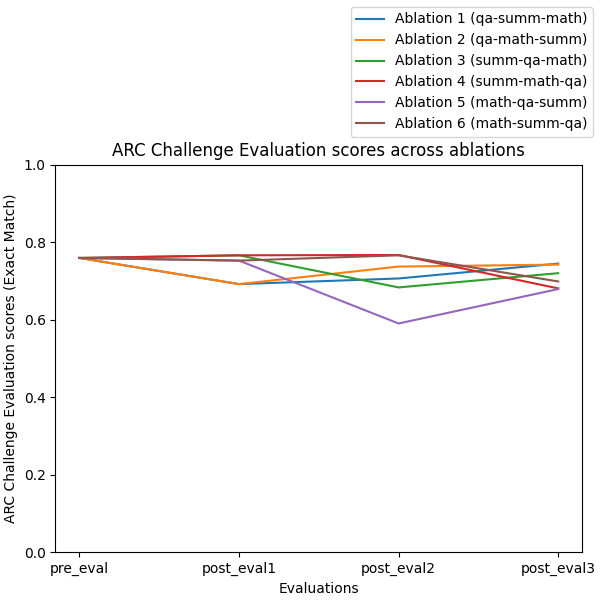
\includegraphics[width=1.1\textwidth]{Figures/results/trace_baseline_graphs/arc_challenge/arc_challenge_eval_baseline.png} % first figure itself
        \captionsetup{width=1.1\textwidth}
        \caption{ARC-Challenge: Baseline runs}
        \label{ARCAblationBaseline}
    \end{minipage}\hfill
    \begin{minipage}{0.45\textwidth}
        \centering
        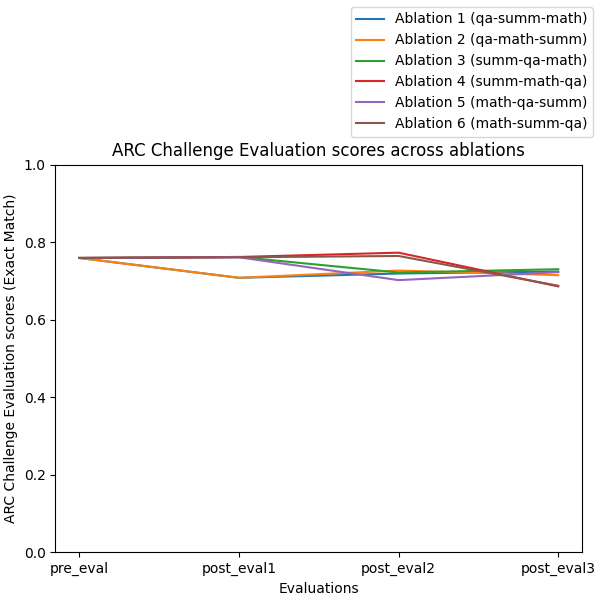
\includegraphics[width=1.1\textwidth]{Figures/results/trace_mitigation_graphs/arc_challenge/arc_challenge_eval_mitigation.png} % second figure itself
        \captionsetup{width=1.1\textwidth}
        \caption{ARC-Challenge: Mitigation runs}
        \label{ARCAblationMitigation}
    \end{minipage}
\end{figure}
The comparison of the model performance on ARC-Challenge benchmark (Figures: \ref{ARCAblationBaseline} and \ref{ARCAblationMitigation}) across different ablations of task order showed that different task sequences yielded different results. This difference in results in the final post-evaluation stage could be an impact of the task order. The variance of the model performance was found to be greater in post\_eval2 for both the baseline and mitigation runs. However, the mitigation runs had more consistent performance across the ablations. 

\begin{figure}[H]
    \centering
    \begin{minipage}{0.45\textwidth}
        \centering
        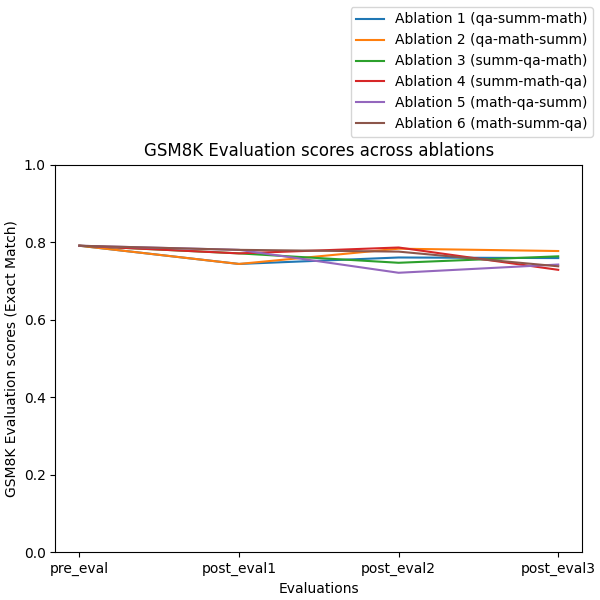
\includegraphics[width=1.1\textwidth]{Figures/results/trace_baseline_graphs/gsm8k/gsm8k_eval_baseline.png}
        \captionsetup{width=1.1\textwidth}
        \caption{GSM8K benchmark: Baseline runs}
        \label{GSM8KBaseline}
    \end{minipage}\hfill
    \begin{minipage}{0.45\textwidth}
        \centering
        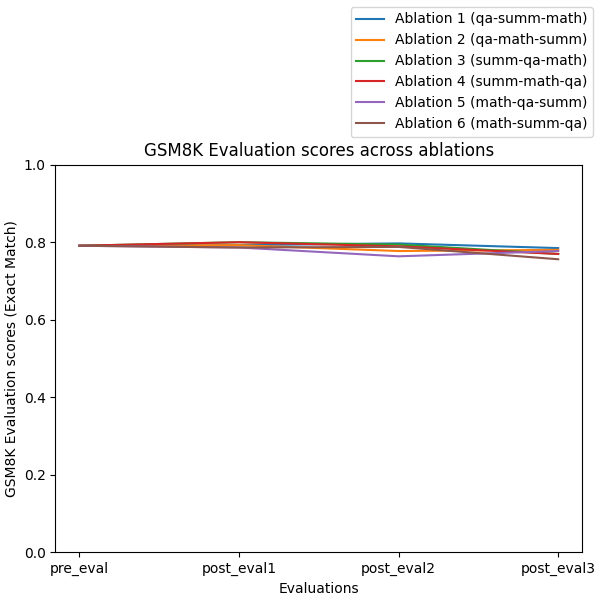
\includegraphics[width=1.1\textwidth]{Figures/results/trace_mitigation_graphs/gsm8k/gsm8k_eval_mitigation.png}
        \captionsetup{width=1.1\textwidth}
        \caption{GSM8K benchmark: Mitigation runs}
        \label{GSM8KMitigation}
    \end{minipage}
\end{figure}

The comparison across task ablations for the GSM8K benchmark (Figures: \ref{GSM8KBaseline} and \ref{GSM8KMitigation}) showed that the task performance did not exhibit much variance across the different ablations, and the task performance remained steady across the post-evaluation stages. The performance across ablations was found to be more consistent for the mitigation runs than for the baseline runs.

\begin{figure}[H]
    \centering
    \begin{minipage}{0.45\textwidth}
        \centering
        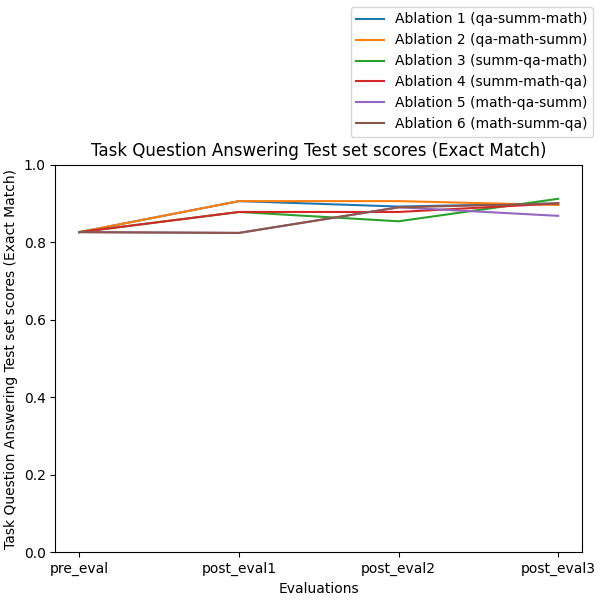
\includegraphics[width=1.1\textwidth]{Figures/results/trace_baseline_graphs/task_eval/qa_test_Test_baseline.png} % first figure itself
        \captionsetup{width=1.1\textwidth}
        \caption{Question Answering Test set: Baseline runs}
        \label{QATestBaseline}
    \end{minipage}\hfill
    \begin{minipage}{0.45\textwidth}
        \centering
        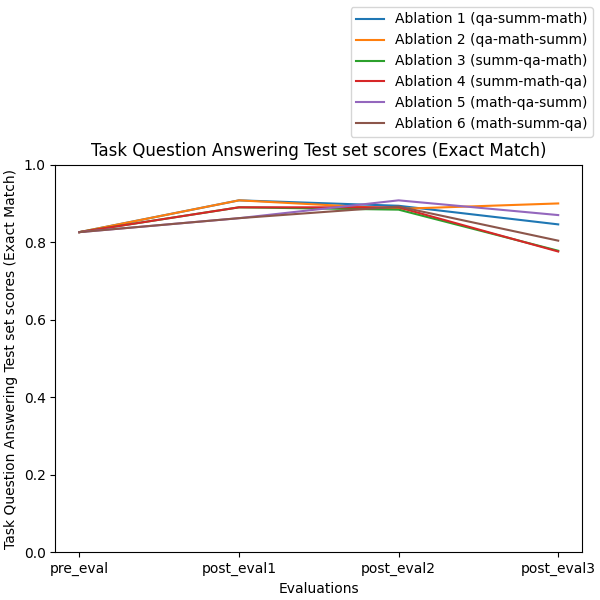
\includegraphics[width=1.1\textwidth]{Figures/results/trace_mitigation_graphs/task_eval/qa_test_Test_mitigation.png} % first figure itself
        \captionsetup{width=1.1\textwidth}
        \caption{Question Answering Test set: Mitigation runs}
        \label{QATestMitigation}
    \end{minipage}
\end{figure}

\begin{figure}[H]
    \centering
    \begin{minipage}{0.45\textwidth}
        \centering
        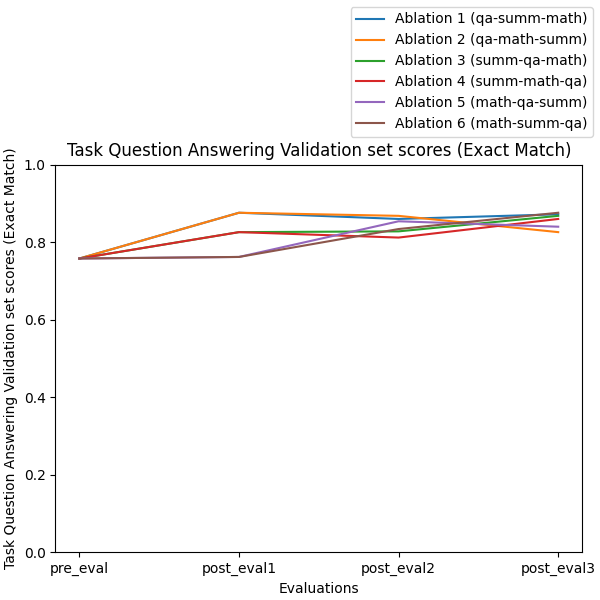
\includegraphics[width=1.1\textwidth]{Figures/results/trace_baseline_graphs/task_eval/qa_val_Validation_baseline.png} % first figure itself
        \captionsetup{width=1.1\textwidth}
        \caption{Question Answering Validation set: Baseline runs}
        \label{QAValBaseline}
    \end{minipage}\hfill
    \begin{minipage}{0.45\textwidth}
        \centering
        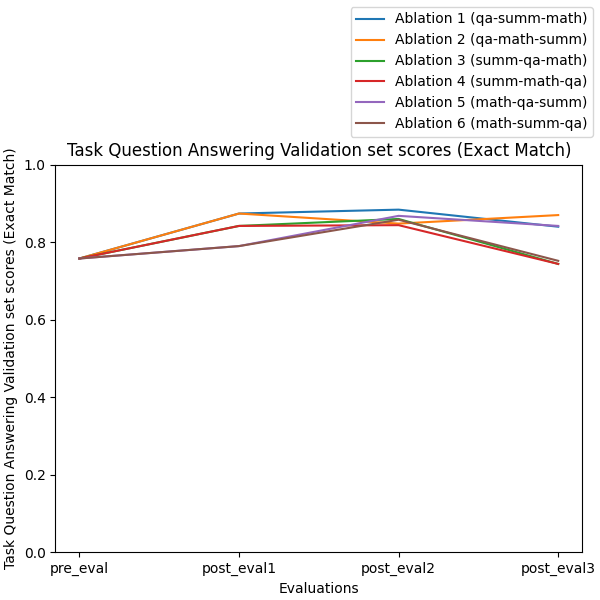
\includegraphics[width=1.1\textwidth]{Figures/results/trace_mitigation_graphs/task_eval/qa_val_Validation_mitigation.png} % first figure itself
        \captionsetup{width=1.1\textwidth}
        \caption{Question Answering Validation set: Mitigation runs}
        \label{QAValMitigation}
    \end{minipage}
\end{figure}

The comparison of the model performance on qa task (Figures: \ref{QATestBaseline}, \ref{QATestMitigation}, \ref{QAValBaseline} and \ref{QAValMitigation}) across the different ablations showed that the performance scores did not vary much across ablations. We observed a difference in the results in post\_eval1 for both the test and validation runs. The performance at the final post-evaluation stage, however, showed different trends in the baseline and mitigation runs. In the baseline run, the performance across different ablations appeared to converge to a similar score in post\_eval3 for both the test and validation sets. However, in the mitigation run, the performance scores appeared to converge in post\_eval2 but then diverged to different values in post\_eval3. 

\begin{figure}[H]
    \centering
    \begin{minipage}{0.45\textwidth}
        \centering
        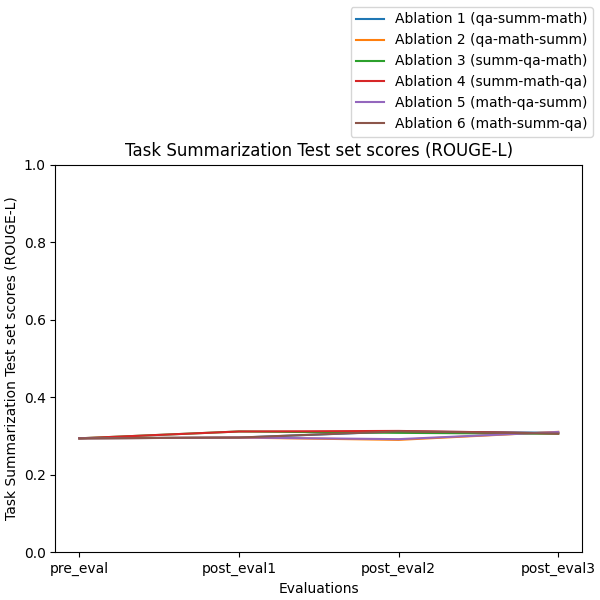
\includegraphics[width=1.1\textwidth]{Figures/results/trace_baseline_graphs/task_eval/summ_test_Test_baseline.png} % first figure itself
        \captionsetup{width=1.1\textwidth}
        \caption{Summarization Test set: Baseline runs}
        \label{SummTestBaseline}
    \end{minipage}\hfill
    \begin{minipage}{0.45\textwidth}
        \centering
        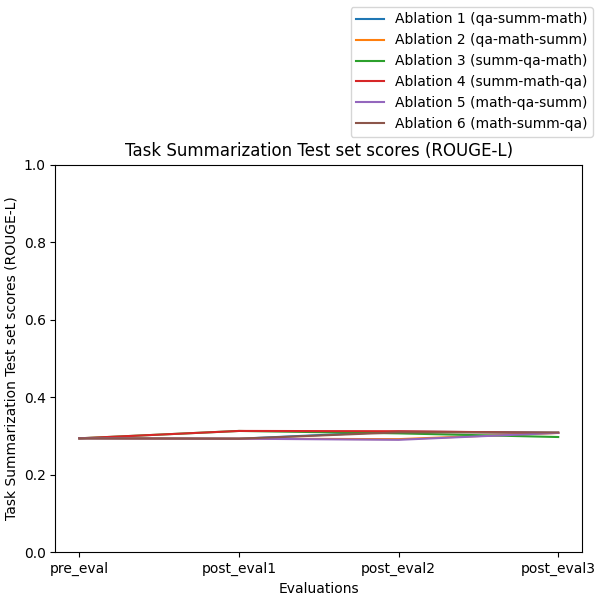
\includegraphics[width=1.1\textwidth]{Figures/results/trace_mitigation_graphs/task_eval/summ_test_Test_mitigation.png} % first figure itself
        \captionsetup{width=1.1\textwidth}
        \caption{Summarization Test set: Mitigation runs}
        \label{SummTestMitigation}
    \end{minipage}
\end{figure}

\begin{figure}[H]
    \centering
    \begin{minipage}{0.45\textwidth}
        \centering
        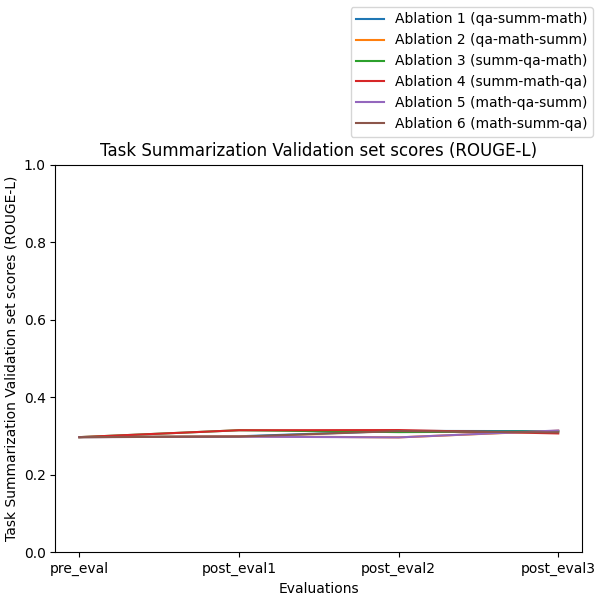
\includegraphics[width=1.1\textwidth]{Figures/results/trace_baseline_graphs/task_eval/summ_val_Validation_baseline.png} % first figure itself
        \captionsetup{width=1.1\textwidth}
        \caption{Summarization Validation set: Baseline runs}
        \label{SummValBaseline}
    \end{minipage}\hfill
    \begin{minipage}{0.45\textwidth}
        \centering
        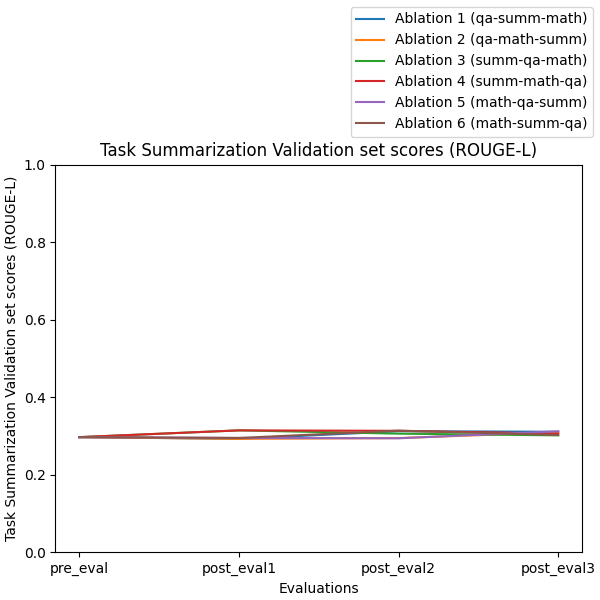
\includegraphics[width=1.1\textwidth]{Figures/results/trace_mitigation_graphs/task_eval/summ_val_Validation_mitigation.png} % first figure itself
        \captionsetup{width=1.1\textwidth}
        \caption{Summarization Validation set: Mitigation runs}
        \label{SummValMitigation}
    \end{minipage}
\end{figure}
The comparison of the model performance across different ablations for summ task (Figures: \ref{SummTestBaseline}, \ref{SummTestMitigation}, \ref{SummValBaseline} and \ref{SummValMitigation}) showed that the model performance remained consistent across the different ablations. This trend was observed for both the test and validation set in both the baseline and mitigation runs. 

\begin{figure}[H]
    \centering
    \begin{minipage}{0.45\textwidth}
        \centering
        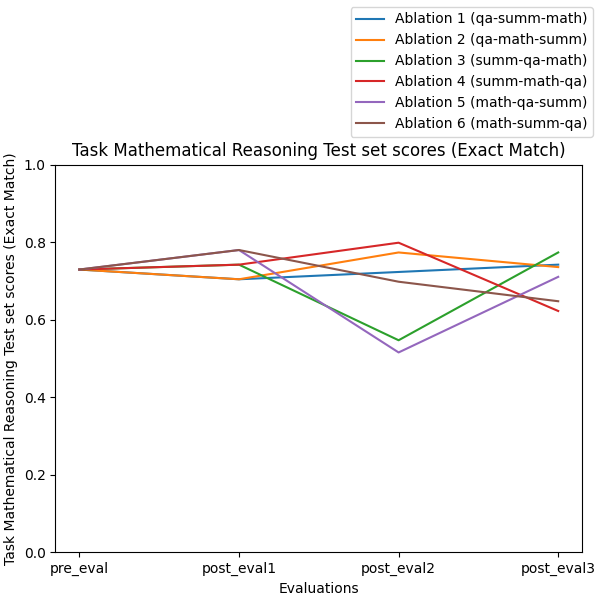
\includegraphics[width=1.1\textwidth]{Figures/results/trace_baseline_graphs/task_eval/math_test_Test_baseline.png} % first figure itself
        \captionsetup{width=1.1\textwidth}
        \caption{Mathematical Reasoning Test set: Baseline runs}
        \label{MathAblationBaseline}
    \end{minipage}\hfill
    \begin{minipage}{0.45\textwidth}
        \centering
        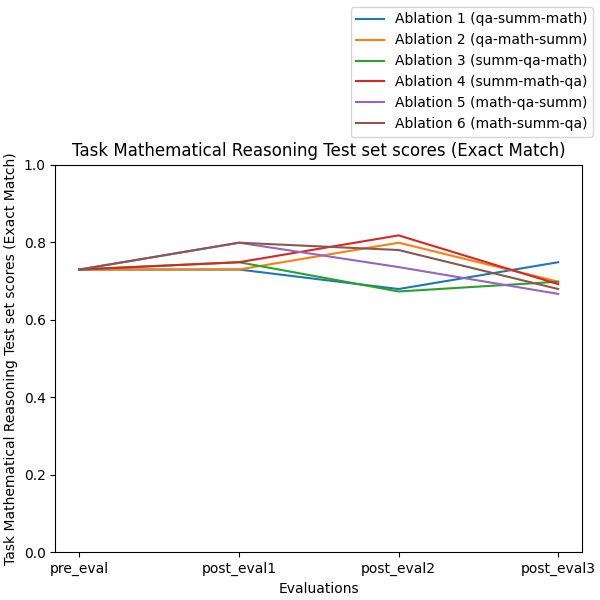
\includegraphics[width=1.1\textwidth]{Figures/results/trace_mitigation_graphs/task_eval/math_test_Test_mitigation.png} % first figure itself
        \captionsetup{width=1.1\textwidth}
        \caption{Mathematical Reasoning Test set: Mitigation runs}
        \label{MathAblationMitigation}
    \end{minipage}
\end{figure}

\begin{figure}[H]
    \centering
    \begin{minipage}{0.45\textwidth}
        \centering
        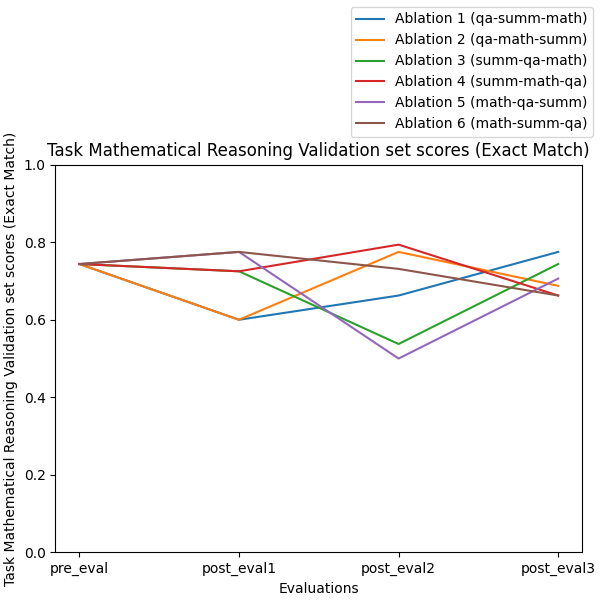
\includegraphics[width=1.1\textwidth]{Figures/results/trace_baseline_graphs/task_eval/math_val_Validation_baseline.png} % first figure itself
        \captionsetup{width=1.1\textwidth}
        \caption{Mathematical Reasoning Validation set: Baseline 
        runs}
        \label{MathAblationValBaseline}
    \end{minipage}\hfill
    \begin{minipage}{0.45\textwidth}
        \centering
        \includegraphics[width=1.1\textwidth]{Figures/results/trace_mitigation_graphs/task_eval/math_val_Validation_mitigation.png} % first figure itself
        \captionsetup{width=1.1\textwidth}
        \caption{Mathematical Reasoning Validation set: Mitigation runs}
        \label{MathAblationValMitigation}
    \end{minipage}
\end{figure}

The comparison of the model performance on the math task across different ablations (Figures: \ref{MathAblationBaseline}, \ref{MathAblationMitigation}, \ref{MathAblationValBaseline}, and \ref{MathAblationValMitigation}) showed that different task sequences led to different results in the final post-evaluation stage. The performance scores appeared to have greater variance in post\_eval2 for both the test and validation sets. In comparing the baseline and mitigation results, we found that the mitigation runs were more steady with fewer inconsistencies across ablations of task order.


\section{Discussion}

\newcommand{\RQone}{How does task-incremental instruction fine-tuning using parameter efficient methods on different tasks influence the retention of the innate capabilities of a pre-trained model:}
\newcommand{\RQonea}{for code pre-trained models in code generation?}

\begin{enumerate}
    \item[\textit{\textbf{RQ1.}}] \textit{\RQone}
    \begin{enumerate}
        \item[\textit{\textbf{RQ1a.}}] \textit{\RQonea}
    \end{enumerate}
\end{enumerate}

To address this research question, we looked at the results of the baseline experiments on the Code Generation use case and focused on the results from the benchmark evaluations. The analysis of the results showed a decline in the performance scores on the benchmark datasets across the post-evaluation stages. The performances on the C++ and Java datasets of the HumanEval (+ MultiPL-E) benchmark were impacted the most with a decline from 0.63 to 0.43 for the C++ dataset and from 0.64 to 0.38 for the Java dataset. The Python dataset of the HumanEval (+ MultiPL-E) benchmark also exhibited a deterioration in performance. However, the performance on the CoNaLa benchmark remained relatively steady throughout the fine-tunes. 

This degradation of model performance on the benchmark datasets indicated forgetting of the model’s innate capabilities. Thus, performing task-incremental instruction fine-tuning using parameter efficient methods on different tasks impacts the innate capabilities of a pre-trained model, resulting in the loss of some pre-trained capabilities. The severity of the impact might be influenced by the nature of the tasks used for fine-tuning and its similarity with the pre-training data of the model. 

\newcommand{\RQoneb}{for general language pre-trained models in terms of reasoning, comprehension, and math?}

\begin{enumerate}
\item  
    \begin{enumerate}
        \item[\textit{\textbf{RQ1b.}}] \textit{\RQoneb}
    \end{enumerate}
\end{enumerate}

For understanding the impact on general language models, we looked at the results of the baseline experiments on the Natural Language Generation use case and focused on the results from the ARC-Challenge and GSM8K benchmarks. The analysis of the results showed a steady decline in the performance scores for both benchmarks over the evaluation stages. The performance on the ARC-Challenge dataset declined from 0.75 to 0.71 and the performance on the GSM8K dataset declined from 0.79 to 0.75 from the pre-evaluation to the final post-evaluation stage. This degradation of performance indicates a loss of the model’s pre-trained capabilities, and thus reaffirms our findings from the Code Generation use case.

\newcommand{\RQtwo}{Do different tasks have varying levels of impact on the retention of the pre-trained model’s capabilities:}
\newcommand{\RQtwoa}{for code models when we train on unseen code, unit-test of unseen code, and manifest generation?}

\begin{enumerate}
    \item[\textit{\textbf{RQ2.}}] \textit{\RQtwo}
    \begin{enumerate}
        \item[\textit{\textbf{RQ2a.}}] \textit{\RQtwoa}
    \end{enumerate}
\end{enumerate}

To address this question, we looked at the baseline experiment results and focused on comparing the pre-evaluation and the 1st post-evaluation scores for the benchmark datasets to check the impact of individual task-specific fine-tuning on the innate capabilities of the model. These experiment results are reported in Section \ref{CodeBaselineExperiments}. 
\begin{enumerate}
\item For HumanEval (+ MultiPL-E) C++ dataset (Table \ref{tab:CppBaseline}), it was observed that utg task training caused the highest decline in performance from 0.63 to 0.3, whereas cg and mg task training caused declines from 0.63 to 0.52 and from 0.63 to 0.54 respectively.
\item For HumanEval (+ MultiPL-E) Java dataset (Table \ref{tab:JavaBaseline}), cg task caused the highest decline for model performance from 0.64 to 0.5. When fine-tuned on utg task, the model performance decreased from 0.64 to 0.54. For the mg task, it was observed that the performance declined from 0.64 to 0.56.
\item For HumanEval (+ MultiPL-E) Python dataset (Table \ref{tab:PythonBaseline}), the model performance got impacted the most by cg task, with a performance decline of 0.76 to 0.67. For utg and mg tasks, the performance declines were from 0.76 to 0.7 and from 0.76 to 0.71 respectively.
\item For the CoNaLa benchmark (Table \ref{tab:CoNaLaBaseline}), it was observed that cg task cause a slight performance decline from 0.216 to 0.212. However, utg and mg task training caused the performance score to increase slightly from 0.216 to 0.22 for both tasks.
\end{enumerate}
These results showed that different tasks have different levels of impact on the innate capabilities of the pre-trained model. 


\newcommand{\RQtwob}{for general language models when we further train on summarization, question answering, and math tasks?}
\begin{enumerate}
\item  
    \begin{enumerate}
        \item[\textit{\textbf{RQ2b.}}] \textit{\RQtwob}
    \end{enumerate}
\end{enumerate}

Similar to RQ2a, we looked at the baseline experiment results and focused on comparing the pre-evaluation and the 1st post-evaluation scores for the ARC-Challenge and GSM8K benchmarks. These experiment results are reported in Section \ref{TraceBaselineExperiments}. 
\begin{enumerate}
\item For ARC-Challenge benchmark, it was observed that qa task training caused the highest decline from 0.759 to 0.69, whereas math task caused a tiny decline from 0.759 to 0.752. The summ task training improved the model performance by a small margin from 0.759 to 0.766.
\item For GSM8K benchmark, it was observed that qa task training cased the highest decline from 0.79 to 0.74, whereas summ and math task training caused slight declines from 0.79 to 0.77 and from 0.79 to 0.78 respectively.
\end{enumerate}

The results on the Natural Language Generation use case reaffirmed our findings on the Code Generation use case that different tasks have different levels of impact on the retention capabilities of pre-trained models.

The varying levels of impact on the retention of the innate capabilities of the model could be a consequence of the nature of the task and the similarity between the data distribution of the task data and the pre-training data of the model. From these observations, we can see that some tasks are more prone to cause catastrophic forgetting of the model’s innate capabilities than others. 

\newcommand{\RQthree}{Does the order in which we perform task-incremental instruction fine-tuning have varying levels of impact on the retention of the pre-trained model’s capabilities:}
\newcommand{\RQthreea}{for code models when we train on unseen code, unit-test of unseen code, and manifest generation?}

\begin{enumerate}
    \item[\textit{\textbf{RQ3.}}] \textit{\RQthree}
    \begin{enumerate}
        \item[\textit{\textbf{RQ3a.}}] \textit{\RQthreea}
    \end{enumerate}
\end{enumerate}

To address this question, we looked at the experiments with the task order ablations for Code Generation use case, discussed in Section \ref{CodeTaskOrderImpact}. To examine the impact on the retention of the innate capabilities of the model, we focused on the HumanEval (+ MultiPL-E) and CoNaLa benchmark evaluation results. From the results, we observed the impact of task order on the performance varied based on the evaluation task. For HumanEval (+ MultiPL-E) C++ and Java datasets, it was observed that the different ablations of task order led to different results in the final post-evaluation stage. For the HumanEval (+ MultiPL-E) Python dataset, it was observed that the performances did not vary much across ablations. The mitigation run for Python had varied results for different task sequences in the final post-evaluation stage. However, for the CoNaLa benchmark, the model performance remained consistent across all ablations for both baseline and mitigation runs. Thus, depending on the evaluation task, task order has varying degrees of impact on the retention of the pre-trained model capabilities.

\newcommand{\RQthreeb}{for general language models when we further train on summarization, question answering, and math tasks?}

\begin{enumerate}
\item  
    \begin{enumerate}
        \item[\textit{\textbf{RQ3b.}}] \textit{\RQthreeb}
    \end{enumerate}
\end{enumerate}

To check if the order in which we perform task-incremental fine-tuning impacts the retention of the model's pre-trained capabilities, we looked at the experiments with the task order ablation for Natural Language Generation use case, discussed in Section \ref{TraceTaskOrderImpact} and focused on the benchmark results. From the results of the benchmark evaluations, we observed that the degree of impact of the task order varies depending on the evaluation task. For the ARC-Challenge, it was observed that different task sequences yielded slightly different results in the final post-evaluation stage for the baseline run. However, the results were similar across ablations for the mitigation runs. For the GSM8K benchmark, it was observed that the task performance did not demonstrate much variance across the different ablations in both the baseline and mitigation runs. Thus, the order in which task-incremental learning is performed has different levels of impact on the different innate capabilities of the model. Some capabilities might experience greater forgetting, depending on the order of tasks that the model is trained on.


\newcommand{\RQfour}{Does the order in which we perform task-incremental instruction fine-tuning have varying levels of impact on the retention of previous tasks’ that are novel to the base model:}
\newcommand{\RQfoura}{for unseen code, unit-test of unseen code, and manifest generation?}

\begin{enumerate}
    \item[\textit{\textbf{RQ4.}}] \textit{\RQfour}
    \begin{enumerate}
        \item[\textit{\textbf{RQ4a.}}] \textit{\RQfoura}
    \end{enumerate}
\end{enumerate}

We explored the experiment results from the task-specific evaluations carried out for the different task sequences on the Code Generation use case (discussed in Section \ref{CodeTaskOrderImpact}) to understand the impact of task order on the previous tasks’ retention capabilities. From the results, we observed that different task orders resulted in different performances at different stages of the task-specific evaluations. For cg task, it was observed that the performance scores show greater variance in post\_eval1 and post\_eval2. However, after the model was trained on all three tasks, the scores were observed to be less varied. This variance, although small, could be attributed to the different task order. For utg task, the different task sequences led to different scores in the final post-evaluation stage. However, for mg task, the final scores converge to a similar value at the final post-evaluation stage. These findings show that the order in which the tasks are sequenced while fine-tuning does have a varying degree of impact on the retention of previous tasks' capabilities. 

\newcommand{\RQfourb}{for summarization, question answering, and math tasks?}

\begin{enumerate}
\item  
    \begin{enumerate}
        \item[\textit{\textbf{RQ4b.}}] \textit{\RQfourb}
    \end{enumerate}
\end{enumerate}

Similar to RQ4a, we explored the experiment results from the task order ablations carried out for Natural Language Generation use case, discussed in Section \ref{TraceTaskOrderImpact}. To understand the impact on the retention of previous tasks’ capabilities, we focused on task-specific evaluations. From the results, it was observed that the performance on summ task remained consistent across the different ablations. For the qa task, the results from the test and validation set did not vary much across ablations. However, the mitigation runs showed that the performance scores varied across ablations in the final post-evaluation stage. The results on the math task showed greater variance across the different task sequences and led to different final scores. From these observations, it is evident that the order in which we perform task-incremental fine-tuning has varying degrees of impact on the retention of task-specific capabilities. 

\newcommand{\RQfive}{Does replay with static buffer size and threshold mitigate forgetting and retain performance when used in task-incremental instruction fine-tuning using parameter-efficient methods:}
\newcommand{\RQfivea}{for the base pre-trained model innate capabilities when the order of training the tasks is varied?}

\begin{enumerate}
    \item[\textit{\textbf{RQ5.}}] \textit{\RQfive}
    \begin{enumerate}
        \item[\textit{\textbf{RQ5a.}}] \textit{\RQfivea}
    \end{enumerate}
\end{enumerate}

To address this question, we looked at the comparisons between the baseline and mitigation runs on the benchmark datasets for both Code Generation and Natural Language Generation use cases. 

\textbf{Code Generation use case}
The comparison of the results of the baseline and mitigation experiments on the benchmark datasets showed that there was a notable decline in performance scores for both the runs and that forgetting still occurred, even with the addition of replay as a mitigation step. From the results, we observed that the mitigation runs demonstrated mixed performance in comparison with the baseline runs. For the HumanEval (+ MultiPL-E) C++ benchmark, the addition of replay provided a small improvement in post\_eval1. Similarly, the mitigation runs had a slight improvement over the baseline runs for the HumanEval (+ MultiPL-E) Java benchmark. However, for the HumanEval (+ MultiPL-E) Python benchmark, the mitigation runs demonstrated a similar or worse performance than the baseline runs. For the CoNaLa benchmark, the addition of replay did not make any impact and the performance remained stable across the evaluation stages.

From these results, we found that replay was not very effective at mitigating forgetting of the base pre-trained model's innate capabilities and the improvements it offered over the baseline approach were small and inconsistent for the benchmark tasks.

\textbf{Natural Language Generation use case}

Upon comparing the results of the baseline and mitigation experiments on the benchmark datasets of the Natural Language use case, it was observed that there was a degradation in the performance across the post-evaluation stages, even with the addition of replay as a mitigation step, for both the benchmarks. For the ARC-Challenge benchmark, the addition of replay provided a slight boost over the baseline runs for post\_eval1 and post\_eval2. However, in the final post-evaluation stage, both runs produced the same result. For GSM8K benchmark, the addition of replay provided slight improvements over the baseline scores across all post-evaluation stages, slightly reducing the severity of forgetting of the model's capabilities. It was observed that the mitigation runs provided a more stable and consistent performance over the baseline runs. On comparing the standard deviations between baseline and mitigation runs, we found that the standard deviations for both benchmarks were lower in all the post-evaluation stages for the mitigation runs.

Thus, the addition of the replay mitigation step was found to not mitigate forgetting completely, but the degree of forgetting of the model's pre-trained capabilities was observed to be slightly reduced. Furthermore, the addition of replay mitigation was found to lead to more stable and consistent performance.

\newcommand{\RQfiveb}{for the subsequent merged new tasks when the order of training the tasks is varied?}

\begin{enumerate}
\item  
    \begin{enumerate}
        \item[\textit{\textbf{RQ5b.}}] \textit{\RQfiveb}
    \end{enumerate}
\end{enumerate}

To address this question, we looked at the comparisons between the baseline and mitigation runs on the task-specific evaluations for both Code Generation and Natural Language Generation use cases. 

\textbf{Code Generation use case}

The comparison of the baseline and mitigation experiments on the task-specific evaluations showed that for both the baseline and mitigation runs, the task-specific performance improved across the post-evaluation stages. For cg task, it was observed that the mitigation run showed very slight improvement over the baseline runs on both test and validation sets. For utg task, the performance was observed to remain steady across the different post-evaluation stages, with the mitigation runs offering a tiny improvement over the baseline runs. The results from mg task showed that the inclusion of replay offered slight improvements in performance in post\_eval1 and post\_eval2. However, the baseline run slightly outperformed the mitigation run in the final post-evaluation stage. 
On comparing the baseline and mitigation runs for consistency, the standard deviations were found to be generally lower for the mitigation runs than for the baseline runs.

Thus, the addition of the mitigation step did not make a significant improvement over the baseline performance. However, we noted that the inclusion of replay mitigation leads to more stable and consistent performance across different orders of tasks.

\textbf{Natural Language Generation use case}

The comparison between the baseline and mitigation results on the task-specific evaluations showed that the addition of replay provided mixed results. For qa, the mitigation provided a slight improvement in the model performance in post\_eval1 and post\_eval2. However, in the final post-evaluation step, the model performance for the mitigation run degraded more in comparison to the baseline runs. For the summ task, the addition of the mitigation step did not make much impact on the model performance. For the math task, the performance was observed to decline for both baseline and mitigation runs, but the performance in the mitigation run was found to be more stable. On comparing the baseline and mitigation runs for consistency, the standard deviations were found to be lower for the post\_eval1 and post\_eval2 stages of qa task in the mitigation run, but it was found to be higher for post\_eval3. For the summ task, the mitigation runs had more variance than the baseline runs. For the math task, the standard deviations were found to be lower for all post-evaluation stages in the mitigation runs.

Thus, the addition of the mitigation step provided inconsistent results on the task-specific evaluations in the Natural Language use case. The replay mitigation does not provide a significant improvement in the performance scores over the baseline. However, it does lead to more consistent performance.
